\documentclass{fkbook}

% \usepackage{sout}
\usepackage{tikz-cd}

% And so on with definitions!
\newtheoremstyle{snazzydefinition}  % name
    {1.5em}                         % Space above
    {0em}                          % Space below
    {\rmfamily}                     % Body font
    {}                              % Indent amount
    {\scshape}                      % Theorem head font
    {.}                             % Punctuation after theorem head
    {.5em}                          % Space after theorem head
    {}  % Theorem head spec (can be left empty, meaning ‘normal’)

\theoremstyle{snazzydefinition}

\newtheorem{examplex}{Example}

\renewenvironment{example}
  {\pushQED{\oldqed}\renewcommand{\qedsymbol}{$\triangle$}\examplex}
  {\popQED\endexamplex}


\setcounter{tocdepth}{4}
\setcounter{secnumdepth}{4}

\mdtheorem[style=theoremstyle]{joke}{Joke}
\renewpagestyle{main}{
  \sethead{Forest Kobayashi}{\scshape\chaptertitle}{Independent Study Notes}
  \headrule
  \setfoot{December 15th, 2018}{}{\thepage\ of \pageref{LastPage}}
} % odd

\usetikzlibrary{knots}

\usepackage{wasysym}

\begin{document}

\pagestyle{plain}
\frontmatter

\fkauthor{Forest Kobayashi}
\fktitle{Category Theory, Topology, and Knots}
\fksubtitle{Some notes from my Independent Study}
\fkalttitle{(Or: \itshape To All the Proofs I've Loved Before)}
\fkaffiliation{{Department of Mathematics\\}{\itshape Harvey Mudd College\\}}
\fksupervisor{Sam Nelson}
\fksupervisoraffiliation{Department of Mathematics, Claremont McKenna College}

\maketitlepage
\tableofcontents
\mainmatter
\chapter{Introduction}
\pagestyle{main}
\section*{Important Note!!!!!}
These notes are \emph{not} polished, or even necessarily complete. I only
decided to typeset my notes each week if I had spare time after doing readings,
practice problems, and other general prep. They were mainly supposed to serve as
a rough record for what I'd read about, and maybe offer me an opportunity to try
and organize some of my thoughts / intuition. Unfinished sections might abound!

\section*{What is this?}
This is a collection of some of the notes I took over the course of my
Independent Study. The format of the course was something like this: each week,
I'd read a few chapters from some subset of $\{$Categories for the Working
Mathematician (MacLane), A First Course in Algebraic Topology (Kosniowski),
Analysis on Manifolds (Munkres), Quandles: An Introduction to the Algebra of
Knots (Nelson)$\}$. Then, on Fridays, I'd meet with my faculty supervisor (Sam
Nelson) and attempt to give an informal ``lecture'' on the material I'd read
about during the week. I selected this format for the following reasons:
\begin{enumerate}
  \item I figured it would force me to develop my intuition to a point where I
    felt like I could explain the concepts I was learning about
  \item I thought it would also force me to really commit lots of the concepts
    to memory, such that I could talk confidently about them without referencing
    the books
  \item Any amount of practice with math communication is good
\end{enumerate}
Most of which actually ended up panning out! Anyways, I might come back and
re-do a lot of the stuff here at some point in the future, but for now, it's a
bit rough around the edges.
\chapter{Basic Category Theory}
\section{Introduction}
Often in mathematics, we are interested in considering collections of
objects with structure, and how that structure is modified or
preserved when mapping to some other object. Category theory makes
this a little more formal. First, we begin with some definitions.\\

\subsection{Meta-objects}~
\begin{definition}[Metagraph]
  A \emph{metagraph} consists of any collection (note: does not mean a
  set! See \emph{proper classes}) of \emph{objects} $o_1, o_2,
  \ldots$ (not necessarily countable), and \emph{arrows} $a_1, a_2,
  \ldots$, together two operations that allow us to put the two in
  correspondence:\\
\end{definition}
\begin{definition}[Domain \& Codomain]
  \emph{Domain}, which assigns to each arrow $a_i$ an object $o_j =
  \mrm{dom}(a_i)$, and \emph{Codomain}, which assigns to each arrow
  $a_i$ an object $o_k = \mrm{cod}(a_i)$.
\end{definition}

As is convention, we denote the above with one of the following
diagrams:
\begin{figure}[H]
  \centering
  \begin{minipage}{.33\linewidth}
    \[
      a_i : o_j \to o_k
    \]
  \end{minipage}
  \begin{minipage}{.33\linewidth}
    \begin{tikzcd}
      o_j \arrow[r, "a_i"] & o_k
    \end{tikzcd}
  \end{minipage}
  \caption{Equivalent representations of the above}
\end{figure}
Of course, these diagrams can become quite complicated:
\begin{figure}[H]
  \centering
  \begin{tikzcd}
    o_1
    \arrow[drr, bend left, "a_1"]
    \arrow[ddr, bend right, "a_2"]
    \arrow[dr, "a_3"] & & o_2 \arrow[d, "a_8"]& \\
    & o_3 \arrow[r, "a_4"] \arrow[d, "a_5"] \arrow[ur, "a_9"]
    & o_4 \arrow[d, "a_6"] & \\
    & o_5 \arrow[r, "a_7"] & o_6
  \end{tikzcd}
  \caption{Complicated diagram}
\end{figure}
Using these metagraphs, we can construct a \emph{metacategory}:
\begin{definition}[Metacategory]
  A \emph{metacategory} is a metagraph, with the addition of two more
  operations:

  \emph{Identity}, which maps each object to an ``identity'' arrow:
  \[
    id(o) = 1_o : o \to o;
  \]
  \emph{Composition}, which maps a pair of arrows $a_1, a_2$ (with
  $\mrm{\dom(a_1) = \cod(a_2)}$) to a ``composite'' arrow, $a_1 \circ
  a_2$, such that composition is associative:
  \begin{figure}[H]
    \centering
    \begin{tikzcd}
      \dom(a_2) \arrow[rd, "a_2\circ a_1"] \arrow[r, "a_2"] & \cod(a_2) =
      \dom(a_1) \arrow[d, "a_1"]\\
      & \cod(a_1)
    \end{tikzcd}
  \end{figure}
  and for all arrows $a_1
  : o_1 \to o_2$, $a_2 : o_2 \to o_3$, $\exists$ an identity arrow
  $1_{o_2}$ such that
  \begin{figure}[H]
    \centering
    \begin{minipage}{.49\linewidth}
      \centering
      \begin{tikzcd}
        o_1 \arrow[r, "a_1"] \arrow[dr, "a_1"] & o_2
        \arrow[d, "1_{o_2}"]\\
        & o_2
      \end{tikzcd}
    \end{minipage}
    \begin{minipage}{.49\linewidth}
      \centering
      \begin{tikzcd}
        o_2 \arrow[d, "1_{o_2}"] \arrow[dr, "a_2"]& \\
        o_2 \arrow[r, "a_2"]& o_3
      \end{tikzcd}
    \end{minipage}
    \caption{Identity arrows}
  \end{figure}
  commute.
\end{definition}

\subsection{Categories, proper}
In order to actually work with the objects we're used to commonly
seeing in mathematics, we'll have to narrow our scope a bit. Notably,
instead of considering a general \emph{collection} of objects, we'll
instead restrict ourselves to just sets. Hence, we can't consider the
category of all categories, and whatnot. We skip the definition of a
directed graph (``diagram scheme''), and jump straight to categories.
Basically, we summarize the metacategory properties, just specifying
that we're using sets now:

\begin{definition}[Category]
  A \emph{category} $C$ consists of
  \begin{enumerate}[label=\arabic*)]
    \item A set $\ob(C)$ of \emph{objects},
    \item A set $\homm(C)$ of \emph{arrows},
    \item A function $\mrm{id} : \ob(C) \to \homm(C)$, by $o \mapsto
      1_o$,
    \item And a function $\circ : \homm(C) \times_{\ob(C)} \homm(C)
      \to \homm(C)$ (with $\times_{\ob(C)}$ giving composable pairs)
      with $(a_1, a_2) \mapsto a_1 \circ a_2$
  \end{enumerate}
\end{definition}

A few terms:
\begin{enumerate}
  \item A category with every arrow identity is called
    \emph{discrete}.
  \item A group is a category with just a single object. Here, the
    object really just represents the ``group itself.'' The arrows are
    morphisms, which we can think of as being ``left multiply by $a$''
    or ``right multiply by $a$.''
\end{enumerate}

\subsection{Functors}
One key aspect of category theory that will be of particular interest
to us is how we can translate structure from one space to another.
This is the basis for, among other things, the field of representation
theory. Here, we want to not only to put objects in correspondence
with each other, but also preserve the morphism structure on them. In
this sense, a functor is a morphism of categories.

\begin{definition}[Functor]
  Let $C, D$ be categories, and let $c \in \ob(C)$, $f,g \in
  \homm(C)$. Then call $\mc{F} = (\mc{F}_o, \mc{F}_a)$ a functor if
  \[
    \mc{F}_o : \ob(C) \to \ob(D) \qquad \mc{F}_a : \homm(C) \to
    \homm(D)
  \]
  such that the following essential properties are preserved:
  \begin{enumerate}
    \item $\forall (f : c \to c') \in \homm(C)$, $\mc{F}_a(f) :
      \mc{F}_o(c) \to \mc{F}_o(c')$, with
      \[
        \mc{F}_a(1_{c}) = 1_{\mc{F}_o(c)}
      \]
      and
      \[
        \mc{F}_a(g \circ f) = \mc{F}_a(g) \circ \mc{F}_a(f).
      \]
  \end{enumerate}
\end{definition}
before we go on, let's take a moment to really think what's going on
here in terms of our diagrams. Loosely speaking, we're finding ways of
folding our diagrams in on themselves such that we don't put two pairs
of antiparallel arrows together. This is best expressed with a
picture:
\begin{figure}[H]
  \centering
  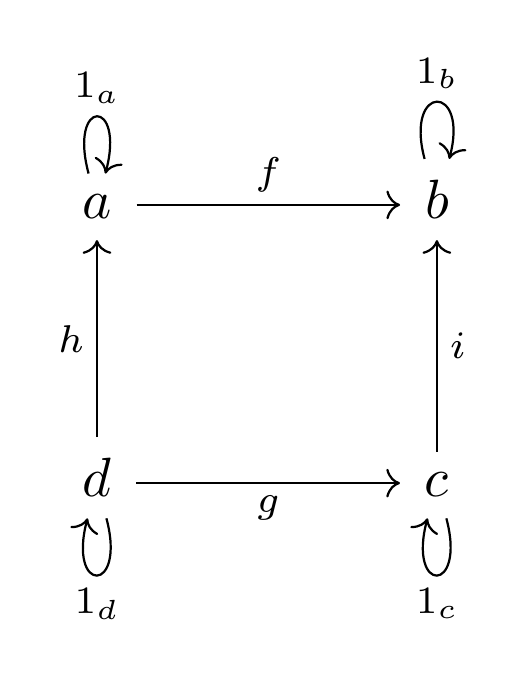
\begin{tikzpicture}
    \node[scale=2] (a) at (0,0) {
      \begin{tikzcd}
        a \arrow[rr, "f"] \arrow[loop above, "1_a"]&  & b
        \arrow[loop above, "1_b"]\\
        &  &  \\
        d \arrow[rr, "g"'] \arrow[uu, "h"] \arrow[loop below,
        "1_d"] &  & c \arrow[uu, "i"'] \arrow[loop below,
        "1_c"]
      \end{tikzcd}
    };
  \end{tikzpicture}
  \caption{Example starting category $C$}
\end{figure}
Suppose we want to map to the following category $D$:
\begin{figure}[H]
  \centering
  \begin{tikzpicture}
    \node[scale=2] (a) at (0,0) {
      \begin{tikzcd}
        &  & c' \arrow[loop above, "1_{c'}"] \\
        & b' \arrow[ru, "g'"] \arrow[loop above, "1_{b'}"] &  \\
        a' \arrow[ru, "f'"] \arrow[loop above, "1_{a'}"]&  &
      \end{tikzcd}
    };
  \end{tikzpicture}
  \caption{Mapped-to category $D$}
\end{figure}
One way we could do so would be to define the following functor:
\begin{align*}
  \mc{F}_o(d) &= a' \\
  \mc{F}_o(a) &= b' \\
  \mc{F}_o(c) &= b' \\
  \mc{F}_o(b) &= c'
\end{align*}
and
\begin{align*}
  \mc{F}_a(1_a) &= 1_{b'} & \mc{F}_a(f) &= g' \\
  \mc{F}_a(1_c) &= 1_{c'} & \mc{F}_a(i) &= g' \\
  \mc{F}_a(1_d) &= 1_{a'} & \mc{F}_a(g) &= f' \\
  \mc{F}_a(1_b) &= 1_{c'} & \mc{F}_a(h) &= f'
\end{align*}
visually, we can interpret this as follows:
\begin{figure}[H]
  \centering
  \begin{tikzpicture}
    \node[scale=.8] (a) at (-7,0) {
      \begin{tikzcd}
        a \arrow[rr, "f"] \arrow[loop above, "1_a"]&  & b
        \arrow[loop above, "1_b"]\\
        &  &  \\
        d \arrow[rr, "g"'] \arrow[uu, "h"] \arrow[loop below,
        "1_d"] &  & c \arrow[uu, "i"'] \arrow[loop below,
        "1_c"]
      \end{tikzcd}
    };

    \node[scale=.8] (b) at (0,0) {
      \begin{tikzcd}
        &  &  & b \arrow[loop above, "1_{b}"] \\
        & a \arrow[rru, "f"] \arrow[loop above, "1_{a}"] &  &  \\
        &  & c \arrow[ruu, "i"'] \arrow[loop below, "1_{c}"] \\
        d \arrow[rru, "g"] \arrow[ruu, "h"] \arrow[loop below,
        "1_{d}"] &  &  &
      \end{tikzcd}
    };

    \draw[dotted, -latex] (-5.5,0) -- (-1.5,0) node[above, midway] {About
      to apply $\mc{F}$};

    \node[scale=.8] (c) at (7,0) {
      \begin{tikzcd}
        &  & c' \arrow[loop above, "1_{c'}"] \\
        & b' \arrow[ru, "g'"] \arrow[loop above, "1_{b'}"] &  \\
        a' \arrow[ru, "f'"] \arrow[loop above, "1_{a'}"]&  &
      \end{tikzcd}
    };

    \draw[-latex] (1.5,0) -- (5.5,0) node[above, midway] {Actually
      applying $\mc{F}$};
  \end{tikzpicture}
  \caption{Demonstration of ``folding''}
\end{figure}
Do in ``class'' --- attempt to prove this is a valid way of thinking
about stuff.

Just as we have ``surjective'' and ``injective'' functions, so too do
we have ``full'' and ``faithful'' functors.\\

\begin{definition}
  A functor $\mc{F} : C \to D$ is called \emph{full} if $\forall c,c'
  \in \ob(C)$, $\forall g : \mc{F}_o(c) \to \mc{F}_o(c')$, $\exists f
  : c \to c' \st g = \mc{F}_a(f)$. Note that this is \emph{not} the
  same thing as being surjective with respect to morphisms and
  objects. In the case of objects, it is quite clear that it need not
  be surjective. With respect to morphisms, this is not quite so.
  However it \emph{does} have to be surjective on
  $\homm(\mc{F}_o(\ob(C)))$. Basically, if we forget about all the
  objects with only the identity morphism defined on them (call this
  resulting category $C'$), then fullness requires that $C'$ map to an
  isomorphic directed sub-graph in $D$ under $\mc{F}$.\\
\end{definition}

\begin{definition}
  A functor $\mc{F} : C \to D$ is called \emph{faithful} if $\forall
  c, c' \in C$, $\forall f_1, f_2 : c \to c'$, then $\mc{F}_a(f_1) =
  \mc{F}_a(f_2) : \mc{F}_o(c) \to \mc{F}_o(c')$ implies $f_1 = f_2$.
  Again, $\mc{F}$ need not be injective on $\ob(D)$, $\homm(D)$. The
  object case is fairly apparent, but with respect to morphisms, it's
  again a little more subtle. Essentially, faithfullness is only
  requiring that if we have two morphims \emph{with the same domain
    and codomain} in $C$, we can't ``squish'' them together in $D$.
  However, morphisms with different domains and codomains can be
  assigned to the same morphism in $D$.
\end{definition}

\begin{definition}
  Subcategories are defined as one might expect a subset of objects
  and arrows such that for each arrow, we have both domain and
  codomain, for each object, we have identity arrow, and for each
  composable pair, we have their composite.
\end{definition}

\section{Natural Transformations}
As it turns out, it's turtles all the way down. We now want to discuss
morphsims of functors.

\begin{definition}
  Let $C,D$ be categories, and let $\mc{F}, \mc{G} : C \to D$ be
  functors. Then call $\eta$ a natural transformation if
  \begin{enumerate}[label=\arabic*)]
    \item $\forall c \in C$, $\eta$ assigns to $c$ a morphism $\eta_c
      : \mc{F}_o(c) \to \mc{G}_o(c)$, called the \emph{component} of
      $\eta$ at $c$. This $\eta_c$ must satisfy
    \item $\forall f : c \to c'$, we have that $\eta_{c'} \circ
      \mc{F}_a(f) = \mc{G}_a(f) \circ \eta_c$
      \begin{figure}[H]
        \centering
        \begin{tikzcd}
          \mc{F}_o(c) \arrow[rr, "\eta_c"] \arrow[dd, "\mc{F}_a(f)"'] &
          & \mc{G}_o(c) \arrow[dd, "\mc{G}_a(f)"] \\
          &  &  \\
          \mc{F}_o(c') \arrow[rr, "\eta_{c'}"] &  & \mc{G}_o(c')
        \end{tikzcd}
        \caption{Natural transformation}
      \end{figure}
  \end{enumerate}
\end{definition}
Essentially, this ``glues'' diagrams of functors together such that
moving around the ``image'' one the $\mc{F}$ side and then hopping
over to the $\mc{G}$ side leaves you in the same place as first
hopping over to the $\mc{G}$ side and then taking an analogous path
there (draw on board maybe). If $\eta$ is invertible (that is, if
every component of $\eta$ is invertible), then we call $\eta$ a
\emph{natural isomorphism} or \emph{natural equivalence}.

Example: determinants, ring homomorphisms, and matrices. Can either
apply (matrix) ring homomorphism first, then take det, or take det,
then apply ring (matrix entries) homomorphism. Either gets the same
result.

\section{Monics, Epics, and Zeros.}
Epic indeed. One might be wondering, \emph{how the heck does this
  whole ``groups as categories with one objec'' thing play out? How do
we distinguish between two morphisms, if they have the same domain and
codomain?} All fantastic questions. Let's jump right into it.

In category theory, our primary focus will largely be on
\emph{morphisms}. As MacLane states, this is part of the power of
Category Theory --- instead of thinking about properties in terms of
element-by-element treatments, we can instead think of them in terms
of morphisms that sort of ``take us between states.'' hence, we bring
a slew of definitions.\\

\begin{definition}[Invertible morphisms]
  Let $C$ a category, and $f : c \to c' \in \homm(C)$. Call $f$
  \emph{invertible} if $\exists f^{-1} : c' \to c \in \homm(C) \st
  f\circ f^{-1} = 1_{c'}$, and $f^{-1} \circ f = 1_c$. Then $f^{-1}$
  is unique, and $f, f^{-1}$ are called \emph{isomorphisms}.\\
\end{definition}
\begin{definition}[Isomorphism]
  Call $c, c' \in \ob(C)$ \emph{isomorphic} if there is an isomorphism
  between them.\\
\end{definition}
\begin{definition}[Monic]
  Let $a,c,c' \in \ob(C)$, and let $m \in \homm_C(c', a)$. Call $m$
  \emph{monic} if $\forall f_1, f_2 \in \homm_C(c,c')$, $m \circ f_1 =
  m \circ f_2 \implies f_1 = f_2$. Basically, $m$ never jumbles up
  parallel arrows from $c$ to $c'$, provided you apply it \emph{after}
  the arrows. It is always \emph{left}-cancellable, and sort of
  ``always preserves information in the domain.''\\
\end{definition}
\begin{definition}[Epi]
  Epis are defined similarly, but are \emph{right}-cancellable. In
  some sense, it never loses information in the co-domain.\\
\end{definition}
\begin{definition}[Right \& Left Inverses]
  Right and left inverses are defined in the expected manner. Let $C$
  a category, and $f \in \homm_C(c,c')$. Then $s \in \homm_C(c', c)$
  is called a \emph{right} inverse or \emph{section} of $f$ if $f\circ
  s = 1_{c'}$, and a \emph{left} inverse or \emph{retraction} if
  $s\circ f = 1_c$. \\
\end{definition}
If $f$ has a right inverse, it is epi, if it has a left inverse, it is
monic. However the converse of these statements do not necessarily
hold. Am still slightly confused about that; remember to ask Prof.
Nelson.

Let $g \in \homm_C(c',c)$, $h \in \homm_C(c,c')$. Then if $g\circ h =
1_c$, call $g$ a \emph{split epi}, $h$ a \emph{split monic}, and $f =
h\circ g$, call $f$ idempotent.

\begin{definition}[Terminal]
  Call an object $c$ \emph{terminal} if $\forall c' \in \ob(C)$,
  $\exists ! f : c' \to c$. \\
\end{definition}

\begin{definition}[Initial]
  Call an object $c$ \emph{initial} if $\forall c' \in \ob(C)$,
  $\exists ! f : c \to c'$. \\
\end{definition}

\begin{definition}[Null]
  Call an object $c$ \emph{null} if it is both initial and terminal.
\end{definition}

\chapter{Duality in Category Theory}
\begin{adjustwidth}{1em}{1em}
  \section{Introduction}
  First, we'll talk about about some of the hom-set stuff we didn't
  really get much time to touch on last time.
  \subsection{Hom-Sets}
  As as we will see, \emph{hom-sets} play a big role in understanding
  functors. For example, calling a functor \emph{full} is equivalent
  to it being \emph{surjective} on a particular hom-set, and similar
  with faithful functors and injectivity.
  \begin{definition}[Hom-set]
    Let $\mb{C}$ be a category, and $a,b \in \ob(\mb{C})$. Then define
    the \emph{hom-set} of $(a,b)$ by
    \[
      \homm_{\mb{C}}(a,b) = \set{f \mid f \in \homm(\mb{C}),\ f : a
        \to b}.
    \]
  \end{definition}
  This suggests the following (equivalent) formulation of the category
  theory axioms:
  \begin{leftbar}
    {\large \bfseries Category Axioms (hom-set version)}
    \begin{enumerate}[label=(\roman*)]
      \item A small \emph{category} is a set of objects $a,b,c,\ldots$
        together with
      \item A function that assigns to each ordered pair $\ip{a,b}$ a
        set $\homm_{\mb{C}}(a,b)$, and
      \item A function \emph{composition} for each ordered triple
        $\ip{a,b,c}$ with
        \[
          \circ : \homm_{\mb{C}}(b,c) \times \homm_{\mb C}(a,b) \to
          \homm_{\mb C}(a,c)
        \]
      \item For each $b \in \ob(\mb C)$, $\homm_{\mb C}(b,b)$ contains
        at least one element $1_b$ satisfying the ``unit'' axioms
        (see: right / left composition by unit)
      \item Hom-sets are pairwise disjoint. This assures $\mrm{dom},
        \mrm{cod}$ are well-defined for all morphisms.
    \end{enumerate}
  \end{leftbar}
  In this context, we can define a functor in terms of hom-sets:
  \begin{definition}[Functor (redux)]
    Let $\mc{T} : \mb{C} \to \mb{B}$ be defined with the usual object
    functor $\mc{T}_o$, together with a collection of functions
    \[
      \mc{T}^{a,b} : \homm_{\mb C}(a,b) \to \homm_{\mb B}(\mc{T}_o(a),
      \mc{T}_o(b))
    \]
    then $\mc{T}$ is \emph{full} when every such $\mc{T}^{a,b}$ is
    surjective, and \emph{faithful} when injective.
  \end{definition}
  On to duality.
  \section{Duality}
  \subsection{Motivation}
  Recall that last time, we defined functors between categories with
  \[
    \mc{T} : \mb{C} \to \mb{B}
  \]
  if
  \[
    \mc{T} =
    \begin{cases}
      \mc{T}_o : \ob(\mb{C}) \to \ob(\mb{B}) &  \\
      \mc{T}_a : \homm(\mb{C}) \to \homm(\mb{B}) &
    \end{cases}
  \]
  such that for all $c \in \ob(\mb{C})$, $\mc{T}(\id{c}) =
  \id{\mc{T}_o(c)}$, and for all $f,g \in \homm(\mb{C})$, $\mc{T}_a
  (g \circ f) = \mc{T}_a(g) \circ \mc{T}_a(f)$. However, as it turns
  out, this is a bit of a restrictive framework --- we could imagine
  plenty of scenarios in which we might want to study something that
  \emph{almost} looks like a functor, except that
  \[
    \mc{T}_a(g \circ f) = \mc{T}_a(f) \circ \mc{T}_a(g).
  \]
  such an object is called a \emph{contravariant} functor, and we will
  examine them in more depth below. But first, note the fundamental
  similarity between the statements above --- if we had objects
  $a,b,c$ with morphisms $f,g,h$ such that the following diagram
  commutes,
  \begin{figure}[H]
    \centering
    \tikzset{node distance=2cm, auto}
    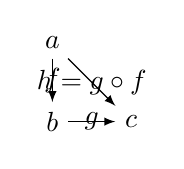
\begin{tikzpicture}
      \node (a) {$a$};
      \node (b) [below of=a] {$b$};
      \node (c) [right of=b] {$c$};
      \draw[-latex] (a) to node {$h = g \circ f$} (c);
      \draw[-latex] (a) to node [swap] {$f$} (b);
      \draw[-latex] (b) to node [swap] {$g$} (c);
    \end{tikzpicture}
    \caption{Example diagram}
  \end{figure}
  then the contravariant functor would create a diagram similar to
  \begin{figure}[H]
    \centering
    \hspace{1.2cm}
    \tikzset{node distance=2cm, auto}
    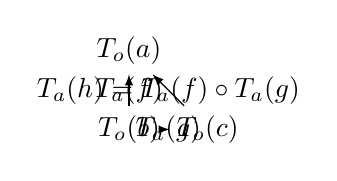
\begin{tikzpicture}
      \node (a) {$\mc{T}_o(a)$};
      \node (b) [below of=a] {$\mc{T}_o(b)$};
      \node (c) [right of=b] {$\mc{T}_o(c)$};
      \draw[-latex] (c) to node [swap] {$\mc{T}_a(h) = \mc{T}_a(f) \circ
        \mc{T}_a(g)$} (a);
      \draw[-latex] (b) to node {$\mc{T}_a(f)$} (a);
      \draw[-latex] (c) to node {$\mc{T}_a(g)$} (b);
    \end{tikzpicture}
    \caption{Example diagram}
  \end{figure}
  certainly these two structures should be thought of as ``similar''
  in some sense --- if there's any justice in the world, we might even
  expect that some theorems we prove about functors in general will
  translate into guarantees about these so-called ``contravariant
  functors.'' Indeed, this is the case: but to make it formal, we need
  to introduce the idea of \emph{duality}, which will prove
  surprisingly powerful.
  \subsection{Basic definitions}
  As you should now expect, we'll build up from axioms:
  \begin{definition}[Atomic Statements]
    Let $\mb{C}$ be a category. Then if $a,b \in \ob(\mb{C})$, $f,g
    \in \homm(\mb{C})$, an \emph{atomic statement} is a statement of
    the form:
    \begin{enumerate}
      \item $a = \dom(f)$ or $b = \cod(f)$
      \item $\id a$ is the identity map on $a$
      \item $g$ can be composed with $f$ to yield $h = g \circ f$.
    \end{enumerate}
    That is, an atomic statement is just a statement about the
    axiomatic properties of categories.
  \end{definition}
  From these, we can build phrases of \emph{statements} using the
  formal grammar defined by propositional logic.
  \begin{definition}[Sentences]
    A \emph{sentence} is a statement (see above) in which we have no
    free variables; that is every variable is ``bound'' or
    ``defined.'' For instance, the statement ``for all $f \in
    \homm(\mc{C})$ there exists $a,b \in \ob(\mc{C})$ with $f : a \to
    b$'' forms a sentence, while ``$f : a \to b$'' is an extreme case
    of one that does not (in the latter, we have no idea what any of
    the variables are actually referring to). In the context of
    category theory, the collection of sentences built out of atomic
    statements are known as \emph{ETAC} (``the elementary theory of an
    abstract category'').
  \end{definition}
  Now, we introduce the concept of \emph{duality}:
  \begin{definition}[Duality]
    Let $\Sigma$ be a statement of ETAC. Then the \emph{dual} of
    $\Sigma$ is intuitively the statement ``in reverse,'' and is
    typically denoted by $\Sigma^*$. This can be formalized as simply
    flipping every ``domain'' statement into a ``codomain'' statement,
    and replacing ``$h = g \circ f$'' with ``$h = f \circ g$.'' Some
    examples of duals are given below:
    \begin{table}[H]
      \centering
      \begin{tabular}{@{}lll@{}}
        \toprule
        Statement $\Sigma$ && Dual Statement $\Sigma^*$ \\ \midrule
        $f : a \to b$ && $f : b \to a$  \\
        $a = \dom(f)$ && $a = \cod(f)$ \\
        $i = \id a$ && $i = \id a$ \\
        $h = g \circ f$ && $h = f \circ g$ \\
        $f$ is monic && $f$ is epic \\
        $u$ is a right inverse of $h$ && $u$ is a left inverse of $h$
        \\
        $f$ is invertible && $f$ is invertible \\
        $t$ is a terminal object && $t$ is an initial object\\
        \bottomrule
      \end{tabular}
    \end{table}
  \end{definition}
  Note that $\Sigma^{**} = \Sigma$, and that if we prove some theorem
  about a statement $\Sigma$, the dual statement $\Sigma^*$ can be
  proven as well.
  \subsection{Contravariance and Opposites}
  We might ask ourselves: what happens if we dual \emph{every}
  statement in $\mb{C}$? What would some of the resulting objects'
  properties be? This is the focus of the next section.
  \begin{definition}[Dual Category]
    Let $\mb{C}$ be a category. Then call $\mb C^*$ (also denoted
    $\mb C^{\rm op}$) the \emph{dual} or \emph{opposite} category iff
    for each statement $\Sigma$ about $\mb C$, $\Sigma^*$ holds about
    $\mb C^*$.
  \end{definition}
  This results in the following properties:
  \begin{leftbar}
    {\large \bfseries Properties of the Dual Category}
    \begin{enumerate}[label=\arabic*)]
      \item $\mb C$ and $\mb C^*$ have the same objects.
      \item We can put each $f \in \homm(\mb C)$ into a one-to-one
        relationship with $f^* \in \homm(\mb C^*)$.
      \item For each $f \in \homm(\mb C)$, $\dom(f) = \cod(f^*)$, and
        $\cod(f) = \dom(f^*)$.
      \item For composable $g,f$, $(g \circ f)^* = f^* \circ g^*$.
      \item If $\Sigma^*$ is true in $\mb C$, then $\Sigma$ is true in
        $\mb C^*$.
    \end{enumerate}
  \end{leftbar}
  Recall our definition of contravariant functors on page 2. The
  important quality that we saw with contravariant functors was that
  they \emph{reverse the order} of morphism composition. One might
  note that this sounds an awful lot like a dual property --- and
  indeed, there is a connection here. We examine this in the theorem
  below.
  \begin{theorem}[Contravariant functors and duality]
    Let $\mb C, \mb B$ be categories, and let $T : \mb C \to \mb B$ be
    a contravariant functor. Then $T$ can be expressed as a covariant
    functor from $\mb C^* \to \mb B$
  \end{theorem}
  \begin{proof}
    Let $a,b,c \in \ob(\mb C)$, and let $f : a \to b$, $g : b \to c$.
    Then if $\mc T : \mb C \to \mb B$ is a contravariant functor, let
    $\ol{\mc T} : \mb C^* \to \mb B$ be defined by
    \[
      \mc T f = \ol{\mc T} f^*
    \]
    for all $f \in \homm(\mb C)$. Then note that
    \begin{align*}
      \mc T(g \circ f)
      &= \ol{\mc T} ((g \circ f)^*) \\
      \mc T(f) \circ \mc T(g)
      &= \ol{\mc T} (f^* \circ g^*) \\
      &= \ol{T}(f^*) \circ \ol{T}(g^*)
    \end{align*}
    thus, $\ol{\mc T}$ is a covariant functor from $\mb C^*$ to $\mb
    B$.
  \end{proof}
  similarly, by the principle of duality, any covariant functor from
  $\mb C \to \mb B$ can be thought of as a contravariant functor from
  $\mb C^* \to \mb B$.

  We look at an interesting example:
  \begin{definition}[Hom-functors]
    Let $\mb C$ be a category with small hom-sets. Then since each
    hom-set is small, for every $a \in \ob(\mb C)$, define the
    \emph{covariant hom-functor}
    \[
      \homm_{\mb C}(a, -): \mb C \to \textbf{Set}
    \]
    such that the object function gives
    \[
      b \mapsto \homm_{\mb C}(a,b)
    \]
    and arrow function
    \[
      \bk{k : b \to b'} \mapsto \bk[Big]{\homm_{\mb C}(a,k) :
        \homm_{\mb C}(a,b) \to \homm_{\mb C}(a, b')}
    \]
    where the RHS of the above is defined by $f \mapsto k \circ f$ for
    each $f : a \to b$. Since the notation above is cumbersome,
    MacLane suggests instead using $k_\star$ (``composition with $k$ on
    the left'', or ``the map induced by $k$'').

    Similarly, we define the \emph{contravariant hom-functor} by, for
    each $b \in \ob{\mb C}$,
    \[
      \homm_{\mb C}(-,b) : \mb C^* \to \textbf{Set}
    \]
    with arrow function
    \[
      \bk{g : a \to a'} \mapsto \bk[Big]{\homm_{\mb C}(g, b) :
        \homm_{\mb C}(a',b) \to \homm_{\mb C}(a, b)}
    \]
    defined by $f \mapsto f \circ g$. Again, omitting $b$, this is
    often written as $g^\star$. In summary,
    \[
      k_\star f = k \circ f \qquad g^\star f = f \circ g
    \]
    and the following diagram commutes.
    \begin{figure}[H]
      \centering
      \tikzset{node distance=3cm, auto}
      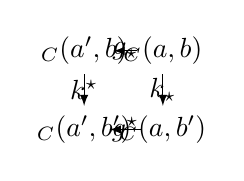
\begin{tikzpicture}
        \node (a) {$\homm_{\mb C}(a', b)$};
        \node (b) [right of=a] {$\homm_{\mb C}(a,b)$};
        \node (c) [below of=a] {$\homm_{\mb C}(a',b')$};
        \node (d) [below of=b] {$\homm_{\mb C}(a,b')$};
        \draw[-latex] (a) to node [swap] {$k^\star$} (c);
        \draw[-latex] (a) to node {$g_\star$} (b);
        \draw[-latex] (b) to node {$k_\star$} (d);
        \draw[-latex] (c) to node {$g^\star$} (d);
      \end{tikzpicture}
    \end{figure}
  \end{definition}

  \subsection{Products of Categories}
  We define the category analog of the cartesian product:
  \begin{definition}[Product of Categories]
    Let $\mb B, \mb C$ be categories. We construct the \emph{product}
    of $\mb B$ and $\mb C$ as follows:
    \[
      \ob(\mb B \times \mb C) = \ob(\mb B) \times \ob(\mb C)
    \]
    and
    \[
      \homm\pn{\mb B \times \mb C} = \homm\pn{\mb B} \times
      \homm\pn{\mb C}.
    \]
    composition is defined in the obvious manner. For all pairs of
    objects $\ip{b.c}$, $\ip{b', c'}$, $\ip{b'', c''}$, and pairs of
    arrows $\ip{f : b \to b',g : c \to c'}$, $\ip{f' : b' \to b'', g'
      : c' \to c''}$, then if
    \[
      \ip{b,c} \xrightarrow{\ip{f,g}} \ip{b',c'}
      \xrightarrow{\ip{f',g'}} \ip{b'', c''}
    \]
    then we write
    \[
      \ip{f',g'} \circ \ip{f,g} = \ip{f' \circ f, g' \circ g}
    \]
  \end{definition}
  We can define \emph{projection} functors in the obvious manner as
  well:
  \begin{definition}
    Consider functors $P,Q$ with
    \[
      P : \mb B \times \mb C \to \mb B \qquad Q : \mb B \times \mb C
      \to \mb C
    \]
    such that, for all $\ip{f,g} \in \ob(\mb{B \times C}), \homm(\mb{B
    \times C})$,
    \[
      P\ip{f,g} = f, \qquad Q\ip{f,g} = g.
    \]
  \end{definition}
  Here, we will see the first of many descriptions of a ``universal''
  property.
  \begin{theorem}[Look-ahead]
    Let $\mb D$ be a category, and $\mc R$, $\mc T$ be any two
    functors with $\mc R : D \to B$, $\mc T : \mb D \to \mb C$. Then
    $\exists! \mc F : \mb D \to \mb B \times \mb C$ such that the
    following diagram commutes:
    \begin{figure}[H]
      \centering
      \tikzset{node distance=2.5cm, auto}
      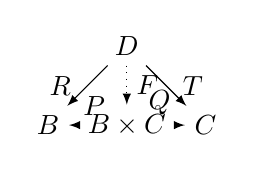
\begin{tikzpicture}
        \node (d) {$\mb D$};
        \node (bc) [below of=d] {$\mb B \times \mb C$};
        \node (b) [left of=bc] {$\mb B$};
        \node (c) [right of=bc] {$\mb C$};
        \draw[-latex] (d) -- (b) node[midway, left, xshift=-.25em] {$\mc R$};
        \draw[-latex] (d) -- (c) node[midway, right, xshift=.25em] {$\mc T$};
        \draw[-latex, dotted] (d) -- (bc) node[midway, right]
        {$\mc F$};
        \draw[-latex] (bc) -- (c) node[midway, above left] {$\mc Q$};
        \draw[-latex] (bc) -- (b) node[midway, above right] {$\mc P$};
      \end{tikzpicture}
      \caption{Uniqueness of inclusion}
    \end{figure}
  \end{theorem}
  \begin{proof} (Sketch) For the diagram to commute, for all $h \in
    \homm(\mb D)$, we must have $\mc F = \ip{\mc R h, \mc T h}$. The
    universality follows pretty trivially.
  \end{proof}
  Similarly to products of categories, we define products of functors:
  \begin{definition}[Functor products]
    Let $\mc U : \mb B \to \mb B'$, $\mc V \to \mb C \to \mb C'$. Then
    we say $\mc U$ and $\mc V$ have a product $\mc U \times \mc V :
    \mb B \times \mb C \to \mb B' \times \mb C'$ if
    \[
      (\mc U \times \mc V)_o(\ip{b,c}) = \ip{\mc U_o a, \mc V_o b} \qquad
      (\mc U \times \mc V)_a(\ip{f,g}) = \ip{\mc U_a f, \mc V_a g}
    \]
    equivalently described by the following commutative diagram:
    \begin{figure}[H]
      \centering
      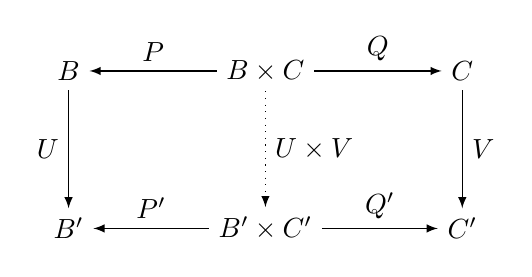
\begin{tikzpicture}
        \node (b) at (-2.5,1) {$\mb B$};
        \node (bc) at (0,1) {$\mb{B \times C}$};
        \node (c) at (2.5,1) {$\mb C$};
        \node (bp) at (-2.5,-1) {$\mb B'$};
        \node (bcp) at (0,-1) {$\mb{B' \times C'}$};
        \node (cp) at (2.5,-1) {$\mb C'$};
        \draw[-latex] (b) -- (bp) node[midway, left] {$\mc U$};
        \draw[-latex, dotted] (bc) -- (bcp) node[midway, right] {$\mc
          U \times \mc V$};
        \draw[-latex] (c) -- (cp) node[midway, right] {$\mc V$};
        \draw[-latex] (bc) -- (c) node[midway, above] {$\mc Q$};
        \draw[-latex] (bc) -- (b) node[midway, above] {$\mc P$};
        \draw[-latex] (bcp) -- (cp) node[midway, above] {$\mc Q'$};
        \draw[-latex] (bcp) -- (bp) node[midway, above] {$\mc P'$};
      \end{tikzpicture}
      \caption{Functor products}
    \end{figure}
  \end{definition}
  Note that since functors are morphisms on categories, then $\times$
  itself is a functor on small categories:
  \[
    \times : \mb{Cat} \times \mb{Cat} \to \mb{Cat}.
  \]
  In the above section, we've concerned ourself with functors mapping
  from a category to a product category (e.g., $\mc F : \mb D \to
  \mb{B \times C}$). We will now examine the ``dual'' concept, that
  functors from a product category to a category.
  \begin{definition}[Bifunctor]
    Let $\mb B$, $\mb C$, $\mb D$ be categories. Let $\mc S : \mb B
    \times \mb C \to \mb D$. Then $\mc S$ is called a
    \emph{bifunctor}.
  \end{definition}
  Simply put, a bifunctor is just a functor of two arguments.

  Let $\mc S$ be the bifunctor given in the definition above. Then if
  we fix one of its arguments, we get something that is effectively a
  single-argument functor, similarly to how fixing an argument of a
  two-variable function yields something that's ``effectively'' a
  single-variable function. This process is described by the following
  theorem:
  \begin{theorem}
    Let $\mb{B}, \mb{C}$, and $\mb{D}$ be categories. For all objects
    $c \in \ob(\mb{C})$ and $b \in \ob(\mb{B})$, let
    \[
      \mc{L}_{c} : \mb{B} \to \mb{D}, \qquad \mc{M}_b : \mb{C} \to
      \mb{D}
    \]
    be functors such that $\mc{M}_b(c) = \mc{L}_c(b)$ for all $b$ and
    $c$. Then there exists a bifunctor $\mc{S} : \mb{B} \times \mb{C}
    \to \mb{D}$ with $S(-, c) = \mc{L}_c$ for all $c$ and $S(b, -) =
    \mc{M}_b$ for all $b$ if and only if for every pair of arrows $f :
    b \to b'$ and $g : c \to c'$ one has
    \begin{equation}
      \mc{M}_{b'}(g) \circ \mc{L}_c(f) = \mc{L}_{c'}(f) \circ
      \mc{M}_b(g) \label{eq:tbd}
    \end{equation}
    These equal arrows \ref{eq:tbd} in $\mb{D}$ are then the value
    $\mc{S}(f,g)$ of the arrow function of $\mc{S}$ at $f$ and $g$.
  \end{theorem}

\end{adjustwidth}


\chapter{Basic Topology}

\begin{center}
  \begin{minipage}[H]{.4\linewidth}
  (Sung to the tune of \emph{Time in a Bottle}) \\
  If I could save Klein in a Bottle \\
  The first thing that I'd like to glue\\\
  Is an edge to an edge\\
  Of a projective plane and then $\#$ \\
  With another $P2$
  \end{minipage}
\end{center}
\section{Introduction}
\begin{adjustwidth}{1em}{1em}
  First, a motivating quote.
  \begin{quote}
    ``Point set topology is a disease from which later generations
    will regard themselves as having recovered'' -Henri Poincar\'{e}
  \end{quote}
  That's\ldots not exactly a ringing endorsement. Why did Henri
  Poincar\'{e} have such a low opinion of point-set topology? Well,
  loosely speaking, because it's just not the right tool for the job,
  especially when compared to \emph{algebraic topology}.

  As it turns out, lots of topics in topology can be simplified by
  attaching algebraic objects to topological spaces, and proving that
  certain properties of this object correspond naturally to properties
  of our topological space. The vehicle by which we navigate between
  the two is, as one might expect, Category Theory. First, we give a
  brief summary of basic concepts in algebraic topology, before moving
  into the Homology presentation given in Matveev.

  \subsection{Basic Point-Set Topology}
  As in most branches of mathematics, our object of study here will be
  some collection of sets, together with some \emph{structure} we can
  associate with them. In Elementary Algebra, this takes the form of
  \emph{group} and \emph{ring} operations, and later the respective
  homomorphisms preserving them. In Elementary Analysis, this (loosely
  speaking) took the form of a \emph{distance metric}, and the
  properties it bestowed on sets. Analogous to our study of
  homomorphisms in Algebra, we often studied \emph{continuous
    functions} in Analysis, and the properties of sets that they
  preserved. Note the resemblance between the two expressions:
  \begin{minipage}[H]{.49\linewidth}
    \begin{figure}[H]
      \centering
      \[
        \varphi(g_1 \oplus g_2) = \varphi(g_1) \otimes \varphi(g_2)
      \]
      \caption*{A homomorphism $\varphi : G \to H$}
    \end{figure}
  \end{minipage}
  \begin{minipage}[H]{.49\linewidth}
    \begin{figure}[H]
      \centering
      \[
        d(x,y) < \delta \implies d'(f(x), f(y)) < \varepsilon
      \]
      \caption*{A continuous function $f : (E,d) \to (E', d')$}
    \end{figure}
  \end{minipage}

  while the analogy doesn't hold exactly, in both cases, we have some
  particular class of functions such that structure in one space is
  preserved in the image. In the case of homomorphisms, the group
  operation in the first group is ``respected'' by the homomorphism
  upon mapping into the second. In the case of continuous functions,
  our equation is essentially stating that the function respects
  things being ``close'' to one another (our map doesn't destroy the
  properties of the distance metric). We can think of this as
  stipulating that we didn't ``tear'' our starting space at all. This
  is best visualized by thinking about our continuous functions not as
  their \emph{graphs} (as we are often used to), but rather as
  \emph{maps} that deform the input domain in various manners to yield
  the image. As an example, one might think of the function $f(x) =
  x^2$ as the action of folding $\RR$ on itself, and stretching the
  edges out towards infinity (this is often a strategy employed in
  visualizing complex-valued functions).

  One might wonder what sorts of interesting discoveries we could make
  by generalizing our starting premises on the right-hand-side, so
  that we could make our questions more similar to those on the left.
  That is, similarly to how we defined distance metrics so as to
  generalize the \emph{key} properties of Euclidean distance, so too
  will we generalize the idea of \emph{continuity of a function}. This
  is the central idea of basic topology. Now, all we need is a good
  place to start. Recall the following theorem of Analysis:
  \begin{theorem}
    Let $(E,d)$ and $(E', d')$ be metric spaces. Then a function $f :
    E \to E'$ is said to be \emph{continuous} iff for all open sets $U
    \subseteq M_2$, we have $f^{-1}(U) \text{ is open in } M_1$.
  \end{theorem}
  Note, this theorem makes no guarantees about the image of an open
  set being open in the codomain. Really, we can make our image as
  ``jagged'' as we want (within reason), provided we fold and deform
  our domain in a smooth manner. But it does indicate to us open sets
  appear to be intimately tied to the idea of ``smooth'' deformations.
  In particular, noting that the theorem is an if and only if, we
  might wonder what would happen were we to discard the distance
  metric entirely, and take the above as a \emph{definition} instead
  of as a \emph{theorem}. There's just one catch: if we really want to
  discard the metric, how are we going to define the notion of an
  ``open'' set? Topologies provide the answer.
  \subsection{Some definitions}~
  \vspace{-.75em}
  \begin{definition}
    Let $X$ be a set, and let $\mc U$ be a collection of subsets of
    $X$ satisfying the following:
    \begin{enumerate}[label=(\roman*)]
      \item $\varnothing \in \mc U$, $X \in \mc U$.
      \item For all $U_1, U_2 \in \mc U$, we have $U_1 \cap U_2 \in
        \mc U$ (by induction, we obtain closure under finite
        intersections).
      \item For any subset $\set{U_i \mid i \in I} \subseteq \mc U$,
        we have
        \[
          \bigcup_{i \in I} U_i = \bm{U} \in \mc U
        \]
        ($\mc U$ is closed under arbitrary unions).
    \end{enumerate}
    then $\mc U$ is called a \emph{topology} for $X$, and $(X, \mc U)$
    is called a \emph{topological space}. We call the elements of $\mc
    U$ the \emph{open sets of} $(X, \mc U)$.
  \end{definition}
  note that a topology is thus a particular kind of \emph{algebra of
    sets} under the binary operations $\cup, \cap$, with identity
  $\varnothing$ for $\cup$, and $X$ for $\cap$. Note that $(\cup,
  \varnothing)$, $(\cap, X)$ are duals of each other, in the sense
  that for any sentence $S$ built out of atomic propositions about our
  set algebra, if $S$ is true, then the statement we obtain by
  \begin{enumerate}[label=\arabic*.]
    \item Replacing each $\cup$ with $\cap$ and each $\cap$ with
      $\cup$,
    \item Interchanging each $\varnothing$ and $X$, and
    \item Reversing inclusions
  \end{enumerate}
  must also be true. Less relevantly (but maybe an object of
  interest), observe that if we replace ``arbitrary unions'' with
  ``countable unions'', and further require closure under
  complementation, then we obtain a $\sigma$-algebra.

  As it turns out, this definition of a topology is more general than
  that given by distance metrics. Whereas every distance metric gives
  rise to a topology, there are topologies that are not
  \emph{metrizable}, meaning they do not arise from any metric on a
  set. We list a few common topologies. Let $(X, \mc U)$ be a
  topological space. Then
  \begin{enumerate}[label=\arabic*.]
    \item If $\mc U = \set{\varnothing, X}$, we call $\mc U$ the
      \emph{concrete} or \emph{indiscrete topology}.
    \item If $\mc U = \mc P(X)$ (i.e., every subset of $X$ is open),
      then we call $\mc U$ the \emph{discrete topology}. Note the
      direct connection to the discrete metric.
    \item Suppose $\mc U = \set{\varnothing, X} \cup \set{U \subseteq
        X \MID \abs{\ol{U}} < \infty}$. That is, $X, \varnothing$, and
      all subsets of $X$ with finite compliment. Then call $\mc U$ the
      \emph{finite complement topology}.
    \item Let $X = \RR$, and $\mc U = \set{\varnothing, \RR} \cup
      \set{(x, \infty) \MID x \in \RR}$
  \end{enumerate}
  As an exercise, I'll give a proof for some of these. Note that
  below, I'll be using overline to denote the compliment of a set, a
  notation I'll discard quickly once we start talking about
  compliments. But for now, it's the most convenient.
  \begin{enumerate}[label=\arabic*.]
    \item Trivial
    \item Also trivial
    \item Observe $\varnothing, X \in \mc U$ by definition. We first
      prove that $\mc U$ is closed under finite intersections. Let
      $U_1, U_2 \in \mc U$. Then $\ol{U_1 \cap U_2} = \ol{U_1} \cup
      \ol{U_2}$ (De Morgan's Laws). The union of two finite sets is
      finite, hence $\ol{U_1 \cap U_2}$ is finite and so $U_1 \cap U_2
      \in \mc U$. Now, let $U' = \set{U_i \mid i \in I} \subseteq \mc
      U$. Then
      \begin{align*}
        \ol{\bigcup_{i \in I} U_i}
        &= \bigcap_{i \in I} \ol{U_i}
      \end{align*}
      which is an intersection of finite sets, and is thust finite
      itself. Hence $\mc U$ is closed under arbitrary unions. It
      follows that $(X, \mc U)$ is a topological space. \qed
    \item The non-trivial elements of $\mc U$ inhereit a total order
      by inclusion from the total order on $\RR$. We add $\varnothing,
      \RR$ to the total order by putting $\RR = \sup (\mc U)$,
      $\varnothing = \inf (\mc U)$. The closure properties follow.
      \qed
  \end{enumerate}
  We define some noteworthy sets.
  \begin{definition}[Interior]
    Let $(X, \mc U)$ be a topological space. Let $Y \subseteq X$. Let
    $U' = \set{U_i \in \mc U \mid i \in I, U_i \subseteq Y}$ be the
    set of all open sets contained in $Y$. Then call the
    \emph{interior} of $Y$ (sometimes denoted $Y^\circ$)
    \[
      \mrm{int}(Y) = \bigcup_{i \in I} U_i.
    \]
  \end{definition}
  we have open sets --- what's next, closed sets???? Yeah, uh, you got
  me there.
  \begin{definition}[Closed sets]
    Let $(X, \mc U)$ be a topological space. Let $C \subseteq X$, and
    let $X - C$ denote the compliment of $C$ in $X$. Then call $C$
    \emph{closed} iff $X - C$ is open. \textbf{VERY VERY IMPORTANT:}
    a set can be both open and closed. In fact, in the discrete
    topology, every set is both.
  \end{definition}
  From the principle of duality (or, alternatively, De Morgan's Laws),
  the dual statements of the topology axioms hold for closed sets.
  That is,
  \begin{enumerate}[label=\roman*.]
    \item $X, \varnothing$ are closed
    \item The set of closed sets is closed (haha) under finite unions
    \item The set of closed sets is closed under arbitrary
      intersections
  \end{enumerate}
  Analogously to the interior of a set, we define its closure. Note
  closure is, in a sense, the dual of the interior
  operator.
  \begin{definition}
    Let $(X, \mc U)$ be a topological space. Let $Y \subseteq X$. Then
    let
    \[
      V' = \set{V_i \mid i \in I, X - V_i \in \mc U, Y \subseteq V_i}
    \]
    that is, the set of all closed sets containing $Y$. Then call the
    \emph{closure} of $Y$ (denoted $\ol{Y}$)
    \[
      \mrm{clos}(Y) = \bigcap_{i \in I} V_i
    \]
  \end{definition}
  Finally, we define the boundary of a set as
  \begin{definition}
    Let $(X, \mc U)$ a topological space. Let $Y \subseteq X$. Then
    define the boundary of $Y$, denoted $\partial Y$, by $\partial Y =
    \ol{Y} - Y$.
  \end{definition}
  One might wonder why we've chosen to recycle the partial derivative
  notation to denote the boundary. The intuitiion is as follows (this
  lightly paraphrased from a stackexchange answer by Terry Tao):
  \begin{leftbar}
    Let $S$ be a smooth, bounded body. Then the surface area
    $\abs{\partial S}$ is the derivative of the volume $\abs{S_r}$ of
    the $r$-neighborhoods $S_r$ at $r = 0$:
    \[
      \abs{\partial S} = \od{}{r} \abs{S_r} \bigg\vert_{r=0}
    \]
    Here's the part I don't understand: he then goes on to say ``More
    generally, one intuitively has the Newton quotient-like formula''
    \[
      \partial S = \lim_{h \to 0^+} \frac{S_h \setminus S}{h}
    \]
    ``the right-hand side does not really make formal sense, but
    certainly one can view $S_h \setminus S$ as a $[0,h]$-bundle over
    $\partial S$ for $h$ sufficiently small (in particular, the radius
    of curvature of $S$).''
  \end{leftbar}
  Finally, we define the neighborhood of a point $x$.
  \begin{definition}[Neighborhood]
    Let $(X, \mc U)$ be a topological space. Let $N \subseteq X$, and
    let $x \in N$. Then call $N$ a neighborhood of $x$ if $x \in
    N^\circ$.
  \end{definition}
  Note the following properties:
  \begin{enumerate}[label=\arabic*.]
    \item $\mrm{clos}$ and $\mrm{int}$ are idempotent.
    \item $X - Y^\circ = \ol{X - Y}$
    \item $\partial Y = \varnothing \iff Y$ is clopen.
    \item Let $U \in \mc U$. Then $Y = \ol{U} \iff Y = \ol{U^\circ}$
      (proof: note $U = U^\circ$).
    \item For each point $x \in X$, there is at least one neighborhood
      of $x$, namely $X$.
    \item If $M$ and $N$ are neighborhoods of $x$, then so is $N \cap
      M$ (use closure under finite intersections).
  \end{enumerate}
  \subsection{Continuous functions and Induced Topologies}
  As promised, we'll now define a continuous function between two
  topological spaces.
  \begin{definition}[Continuous Function]
    A function $f : X \to Y$ between two topological spaces is said to
    be \emph{continuous} if for every open set $U \subset Y$, the
    inverse image $f^{-1}(U)$ is open in $X$ (the same holds for
    closed sets). These are the morphisms in \textbf{Top}.

    If $f$ is bijective with a continuous inverse, then call $f$ a
    \emph{homeomorphism}.
  \end{definition}
  Question: how can we make the following into a trivial statement of
  category theory?
  \begin{leftbar}
    Let $Y$ be a topological space with the property that for every
    topological space $X$, all functions $f : X \to Y$ are continuous.
    Prove that $Y$ has the concrete topology.
  \end{leftbar}
  Answer: use the forgetful functor and the universal mapping
  principle?
  \begin{definition}[Open / closed maps]
    Let $f : X \to Y$. If the image of every open set is open, $f$ is
    said to be \emph{an open map} (define closed maps analogously).
    Note, open mappings are not necessarily continuous.
  \end{definition}
  And lastly, a convenient theorem.
  \begin{theorem}
    Let $(X, \mc U)$, $(Y, \mc V)$ be topological spaces, with $X
    \cong Y$ by a homemorphism $h : X \to Y$. Then for every point $x
    \in X$, $X - \set{x} \cong Y - \set{h(x)}$ (that is, removing a
    point preserves the homeomorphism).
  \end{theorem}
  Intuitively, we think of homeomorphisms as encoding information
  about how two spaces can be stretched and deformed into one another,
  without tearing / gluing pieces together / apart. Note, however,
  that this does not necessarily correspond to our intuitive
  understanding of ``tearing / gluing'' --- were I to hand you a
  circular segment of rope, and ask you to construct the following
  knot
  \begin{figure}[H]
    \centering
    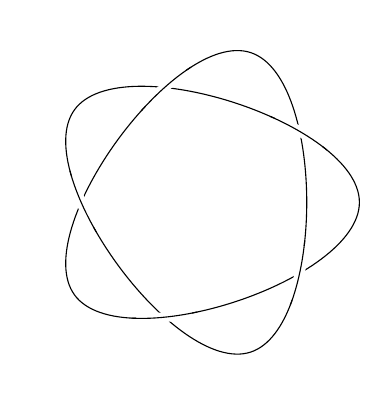
\begin{tikzpicture}
      \begin{knot}[
        consider self intersections=true,
        % draft mode=crossings,
        flip crossing/.list={2,4},
        only when rendering/.style={
          % show curve controls
        }
        ]
        \strand (2,0) .. controls +(0,1.0) and +(54:1.0) .. (144:2) ..
        controls +(54:-1.0) and +(18:-1.0) .. (-72:2) .. controls
        +(18:1.0) and +(162:-1.0) .. (72:2) .. controls +(162:1.0) and
        +(126:1.0) .. (-144:2) .. controls +(126:-1.0) and +(0,-1.0)
        .. (2,0);
      \end{knot}
      % \begin{knot}[
      %   consider self intersections=true,
      %   % draft mode=crossings,
      %   flip crossing/.list={2,4,6}
      %   ]
      %   \strand ([closed]90:2) foreach \k in {1,...,7} { .. (90-360/7+\k*720/7:1.5) .. (90+\k*720/7:2) } (90:2);
      % \end{knot}
    \end{tikzpicture}
    \caption{cinquefoil}
  \end{figure}
  you'd say it couldn't be done. However that's not exactly true. If
  we weren't constrained by the pesky physical details of the real
  world, we could simply pass the rope through itself to yield the
  desired knot. This is what is meant in topology by a homeomorphism
  --- all that has to be conserved are, loosely speaking,
  ``adjacency'' relationships. On the flip side, we might also note
  that this knot can hardly be said to ``not differ at all'' from a
  circle. But in a topological sense, they are homeomorphic. Maybe
  we'll talk about ambient isotopy next week.

  Now, induced topologies. Loosely speaking, this works kind of like a
  group action, except by a topological space on a subset of the
  underlying set. It's worth noting that this analogy might be
  \emph{highly} tenuous.
  \begin{definition}[Induced topologies]
    Let $(X, \mc U)$ be a topological space, and $S \subseteq X$. Let
    $\mc U' = \set{U \cap S \MID U \in \mc U}$. Then we call $\mc U'$
    \emph{the topology on $S$ induced by the topology of $X$} (note
    the desired topological axioms follow from the properties of $\mc
    U$ and the commutativity of union / intersection on sets). If $S$
    has the induced topology, we call $S$ a subspace of $X$.
  \end{definition}
  One thing to note about this definition is that an open set in the
  induced topology need not be open in the original topology. Really,
  what we've essentially done is ``project'' the topological structure
  of some space on to one of its subsets. Naturally, this can't give
  us information about the open-ness of a set selected from $\mc U'$
  were we to imbed it back into $\mc U$. However, if we do know
  something about how $S$ is related to $X$ from the get go,
  \emph{then} we can guarantee a stronger condition:
  \begin{theorem}
    If $S \in \mc U$, then $\mc U' \subseteq \mc U$. That is, the
    opens sets of $S$ are open in $X$. The proof follows directly from
    the definition of induced topology.
  \end{theorem}
  \subsection{Quotient and Product spaces}
  Whereas the induced topology can be thought of as arising from an
  injetive map $\iota : S \to X$, we will now consider the topology
  arising from a surjective map $q : X \to Y$.
  \begin{definition}[Quotient topology]
    Let $f : (X, \mc U) \to Y$ be surjective as a function of sets.
    Then define the \emph{quotient topology} on $Y$ by
    \[
      \mc U' = \set{U \subseteq Y \MID f^{-1}(U) \in \mc U}.
    \]
    The topology axioms follow from properties of the inverse image.
    Once $Y$ has been endowed with the quotient topology, $f$ becomes
    a continuous map.
  \end{definition}
  \begin{theorem}
    Let $f : X \to Y$ be a mapping and suppose that $Y$ has the
    quotient topology with respect to $X$. Let $Z$ be a topological
    space. Then a mapping $g : Y \to Z$ is continuous iff $gf$ is
    continuous.
  \end{theorem}
  In our definition of a quotient topology, because $Y$ is a set
  intially without structure, we don't really care what exactly its
  elements are --- really, all that matters to us is that our mapping
  is surjective ($Y$ only assumes structure once we define the
  quotient topology). Hence, there's no reason why we can't treat all
  such $Y$ as if they were subsets of $X$ (every surjective mapping
  from $X$ to $Y$ can be factored through an isomorphism of $Y$ with a
  subset of $X$). This, together with the suspicious name ``quotient
  topology,'' leads us to question whether we can view this as some
  form of \emph{mod} operation. Indeed, we can. Recall the standard
  definition of an equivalence relation: \clearpage
  \begin{definition}
    Let $X$ be a set. Then an \emph{equivalence relation} $\sim$ is a
    binary relation such that
    \begin{enumerate}
      \item $\sim$ is reflexive,
      \item $\sim$ is symmetric, and
      \item $\sim$ is transitive.
    \end{enumerate}
    For each $x \in X$, we define the \emph{equivalence class of $x$}
    under $\sim$ by $[x] = \set{y \in X \MID x \sim y}$. The set of
    equivalence classes of $X$ under $\sim$ is usually denoted
    $X/\sim$.
  \end{definition}
  For $f : X \to X/\sim$ defined by $f(x) = [x]$, then $X / \sim$
  together with the quotient topology is said to be ``obtained from
  $X$ by topological identification.''

  There is one other way in which we can think about quotient spaces.
  Consider an action on a topological space by a group $G$. Then
  define the equivalence relation $x \sim y \iff y \in \mc{O}_{X}(x)$
  (i.e., they are in the same orbit under the action). Then we can
  give $X/G$ the quotient topology.

  At this point, we've considered various methods of constructing
  topological spaces from existing ones. In the induced topology, we
  thought of giving a set with no structure of its own additional
  structure by including it in a large topological space. In the
  quotient topology, we found ways of taking the structure of a
  topological space and imposing it on some other set. Now, we
  consider the construction in which we have \emph{two} topological
  spaces, and we want to construct a new one from the two.

  \begin{definition}
    Let $(X, \mc U), (Y, \mc V)$ be topological spaces. Define the
    topological product $X \times Y$ by $(X \times Y,\ \mc U \otimes
    \mc V)$, where
    \[
      \mc U \otimes \mc V = \set{\bigcup_{i \in I} W_i \MID i \in I,\
        \text{and}\ W_i \in \mc U \times \mc V}
    \]
    that is, the closure under union of all products of open sets in
    $X$ and $Y$.
  \end{definition}

  \subsection{Compactness and Hausdorffness}
  In analysis, a central question was ``what properties of our spaces
  are preserved under continuous functions?'' To this, we answered
  Completeness, Connectedness, and (in some cases) compactness. Now,
  we'll perform the analogous identification for homeomorphisms. But
  first, we need to define the actual properties we want to prove the
  invariance of. First comes compactness, which I like to think of as
  ``the next-best thing to being finite.''
  \begin{definition}[Covers]
    Let $X$ a set, and let $S \subseteq X$. Then suppose we have $V =
    \set{V_i \subseteq X \MID i \in I}$, and $S \subseteq
    \bigcup_{i\in I} V_i$. Then $V$ is called a \emph{cover} of $S$.
    If $I$ is finite, then we call $V$ a \emph{finite} cover. If $X$
    is a topological space with topology $\mc U$, and $V \subseteq \mc
    U$, then we call $V$ an \emph{open} cover. If we have $V'
    \subseteq V$ a cover of $S$, then we call $V'$ a \emph{subcover}.
  \end{definition}
  now, the familiar definition of compactness. \clearpage
  \begin{definition}
    Let $(X, \mc U)$ a topological space, and let $S \subseteq X$.
    Then $S$ is said to be \emph{compact} if every open cover of $S$
    has a finite subcover.
  \end{definition}
  As one might expect, a subspace $S \subseteq X$ is compact iff it is
  compact under the induced topology.

\end{adjustwidth}

\section{Picking up where we left off}
\begin{adjustwidth}{1em}{1em}
  \subsection{Compactness}
  Last time, we finished by giving some basic definitions of
  comapctness, and whatnot. We'll begin with a small exercise to shake
  some of the cobwebs loose.
  \begin{enumerate}
    \item Suppose that $X$ has the finite complement topology. Show
      that $X$ is compact. Show that each subset of $X$ is compact.
    \item Prove that a topological space is compact if and only if
      whenever $\set{C_j \MID j \in J}$ is a collection of closed sets
      with $\bigcap_{j\in J} C_j = \varnothing$ then there is a finite
      subcollection $\set{C_k \MID k \in K}$ such that $\bigcap_{k \in
        K} C_k = \varnothing$.
    \item Let $\mc F$ be the topology on $\RR$ defined by $U \in \mc
      F$ iff $\forall s \in U, \exists t > s \st [s,t) \subseteq U$.
      Prove that the subset $[0,1]$ of $\mc F$ is not compact.
  \end{enumerate}
  Now
  \begin{enumerate}
    \item Let $U = \set{U_i \mid i \in I}$ be an open cover of $X$.
      Let $U_i \in U$. Then $X - U_i$ is finite. For every $x_j \in X
      - U_i$, $\exists U_j \in U \st x \in U_j$ (because $U$ is a
      cover). Then the set consisting of $U_i$ and the $U_j$ is a
      finite subcover, thus $X$ is compact. Let $Y \subseteq X$. Then
      let $V = \set{V_k \mid k \in K}$ be an open cover of $Y$.
      Proceed an analogous argument to the above to obtain $Y$
      compact.
    \item Let $X$ be a topological space, and suppose $X$ is compact.
      Let $C = \set{C_j \MID j \in J, C_j = \ol{C_j}}$ (i.e., the
      $C_j$ are closed), and suppose
      \[
        \bigcap_{j \in J} C_j = \varnothing.
      \]
      By De Morgan's laws,
      \[
        \bigcup_{j \in J} X - C_j = X
      \]
      since $C_j$ are all closed, then $X - C_j$ are open, hence this
      is an open cover of $X$, and there exists a finite subcover.
      Apply De Morgan's laws again to yield the desired result.
    \item Let $\varepsilon > 0$ be given. Let $U$ be given by the open
      cover
      \[
        U = % \underbrace{
          \set{ \left[ 1 - \frac{1}{2^i}, 1 - \frac{1}{2^{i +
                1}}\right) \MID i = 0, 1, \ldots }% }_{U_1}
      \cup % \underbrace{
        \set{\left[1, 1 + \varepsilon \right)}% }_{U_2},
      \]
      and note that all the sets in $U$ are disjoint, and that they
      cover $[0,1]$. From disjointness, it follows there is no finite
      subcover.
  \end{enumerate}
  \subsection{A brief review of projections}
  On our first pass through, we didn't treat projection maps in a lot
  of depth, so we'll very briefly revisit them here. \clearpage
  \begin{definition}[Projection Maps]
    Let $X, Y$ be topological spaces. Then define $\pi_X : X \times Y
    \to X$, $\pi_Y : X \times Y \to Y$ by
    \[
      \pi_X(x,y) = x \qquad \qquad \pi_Y(x,y) = y
    \]
    $\pi_X$ and $\pi_Y$ are referred to as the \emph{product
      projections}. Note that both are continuous.
  \end{definition}
  \section{Compactness, Continued}~
  \begin{theorem}
    Let $(X, \tau)$ be a topological space, and let $S \subseteq X$.
    Then $S$ is compact in $(X, \tau)$ iff $S$ is compact under the
    induced topology.
  \end{theorem}
  \begin{proof}
    Forwards direction is trivial. For the backwards direction,
    suppose $S$ is compact in the induced topology. Let $U = \set{U_i
      \MID i \in I}$ be an open cover of $S$ in $(X, \tau)$. Then $V =
    \set{V_i = U_i \cap S \MID i \in I}$ is an open cover of $S$ in
    the induced topology, and hence by compactness there exists a
    finite subcover $V' = \set{V_{i_k} \MID i_k \in I, k=1,\ldots,n}$.
    Now, take $U' = \set{U_{i_k} \MID i_k \in I, k =1,\ldots, n}$.
    Then $U'$ is a finite subcover of $U$. Since $U$ was taken to be
    arbitrary, this implies $S$ is comapct.
  \end{proof}
  In the metrizable topologies we encountered in Real Analysis, we
  proved that continuous functions preserve compactness. However, we
  will now show that the same result holds in a general topological
  space.
  \begin{theorem}[Continuity and Compactness]
    Let $f : (X,\tau) \to (Y,\upsilon)$ be a continuous map. Let $S
    \subseteq X$ be a compact subspace. Then $f(S)$ is compact in $Y$.
  \end{theorem}
  \begin{proof}
    Let $V = \set{V_i \mid i \in I} \subseteq \upsilon$ be an open
    cover of $f(S)$. Because $f$ is continuous, $U = \set{f^{-1}(V_i)
      \MID i \in I}$ is a collection of open sets covering
    $f^{-1}(f(S)) \supseteq S$. Since $S$ is compact, there exists a
    finite subcover $U' = \set{f^{-1}(V_{i_k}) \MID i_k \in I, k =
      1,\ldots,n}$ covering $f^{-1}(f(S))$. Then $V' = \set{V_{i_k}
      \mid i_k \in I, k = 1,\ldots,n}$ is a finite subcover of $V$.
    Thus $f(S)$ is compact in $Y$.
  \end{proof}
  By virtue of the properties of continuous functions that we proved
  last time, some nice results follow immediately:
  \begin{corollary}
    ~
    \begin{enumerate}
      \item Any closed interval in $\RR$ is compact.
      \item If $X$ and $Y$ are homeomorphic, then $X$ is compact iff
        $Y$ is.
      \item If $X$ is compact, and $Y$ is any set, then $Y$ with the
        quotient topology induced by $f : X \to Y$ is compact.
    \end{enumerate}
  \end{corollary}
  For completeness, we list some closure properties of compact
  subspaces:
  \begin{theorem}
    Let $(X, \tau)$ be a topological space. Let $S = \set{S_i \MID i
      \in I} \subseteq$ be the collection of compact subspaces of $X$.
    Then
    \begin{enumerate}
      \item If $S_1, S_2 \in S$, then $S_1 \cup S_2 \in S$ (union of
        two compact subspaces is compact). It follows by induction
        that any finite union of compact subspaces is compact.
      \item It is not the case that in an arbitrary topological space,
        an arbitrary intersection of compact spaces is compact (we
        need Hausdorffness). But for finite intersections, things work
        out.
    \end{enumerate}
  \end{theorem}
  % \begin{proof}
  %   \begin{enumerate}
  %     \item Trivial
  %     \item Let
  %       \[
  %         Y = \bigcap_{k \in K} S_k,
  %       \]
  %       where $S_k \in S$, and $K$ is finite. Then let $U = \set{U_i
  %         \mid i \in I}$ be an open cover of $Y$.
  %   \end{enumerate}
  % \end{proof}
  \begin{theorem}
    Let $(X, \tau)$ be a compact topological space, and let $S
    \subseteq X$ be closed. Then $S$ is compact.
  \end{theorem}
  \begin{proof}
    Let $U = \set{U_i \mid i \in I}$ be an open cover of $S$. Let $U_0
    = X - S$. Then $U_0$ is open, and $U \cup \set{U_0}$ covers $X$.
    Then since $X$ is compact, there exists a finite subcover $U' =
    \set{U_i \mid i \in I \cup \set{0}}$. Take $U'' = U' - \set{U_0}$
    to obtain a finite subcover of $U$.
  \end{proof}
  I'm proud to have written this proof without looking at the one in
  the book at all, only to find later that they're basically
  identical.
  \begin{theorem}
    Let $X, Y$ be topological spaces. Then $X, Y$ are compact iff $X
    \times Y$ is compact.
  \end{theorem}
  \begin{proof}~
    \begin{enumerate}
      \item[($\Rightarrow$):] Suppose $X,Y$ are compact. WTS $X \times
        Y$ is compact as well. Let $W = \set{W_i \mid i \in I}$ be an
        open cover of $X \times Y$. Note that $\forall y \in Y$, $X
        \times \set{y}$ is homeomorphic to $X$.
      \item[($\Leftarrow$):] Suppose $X \times Y$ is compact. Let $U =
        \set{U_i \MID i \in I}$ be an open cover of $X$, and $V =
        \set{V_j \MID j \in J}$ be an open cover of $Y$. Then $W$
        given by
        \[
          W = \set{\bigcup_{k \in K} W_k \MID W_k \in U \times V}
        \]
        is an open cover of $X \times Y$, and thus admits a finite
        subcover:
        \[
          W' = \set{W_\ell \mid \ell \in L;\ \abs{L} < \infty}
          \subseteq W
        \]
        Apply a similar trick something something boom
    \end{enumerate}
  \end{proof}
  \section{Hausdorff Spaces}
  Hausdorffness is an important property in Topology that essentially
  allows us to separate things from each other (our space is not
  ``infinitely bunched-up'' somewhere).
  \begin{definition}
    Let $(X, \tau)$ be a topological space. Then call $X$
    \emph{Hausdorff} iff for all $x, y \in X$ such that $x \neq y$,
    there exist open sets $U_x, U_y$ with $x \in U_x$, $y \in U_y$,
    and $U_x \cap U_y = \varnothing$.
  \end{definition}
  Note that by a simple $\varepsilon/2$ argument, it follows that all
  metrizable spaces are Hausdorff.
  \begin{definition}[$T_k$ spaces]
    For $k = 0, 1, 2, 3, 4$, call $X$ a $T_k$ space if it satisfies
    the $k$-th condition below (indexing starts at 0):
    \begin{enumerate}[label=$T_\arabic*$:]
      \item[$T_0$:] For all $x,y \in X$ ($x \neq y$), there is an open
        set $U$ containing one but not the other (i.e., $x \in U$ and
        $y \not \in U$, or $y \in U$ and $x \not \in U$).
      \item For all $x,y \in X$ ($x \neq y$), there are open sets
        $U,V$ such that $x \in U$, $y \in V$, and $x \not \in V$, $y
        \not\in U$.
      \item For all $x,y$ in $X$ ($x \neq y$), there are open sets $U,
        V$ such that $x \in U$, $y \in V$, and $U \cap V =
        \varnothing$ (there are disjoint neighborhoods about $x$ and
        $y$).
      \item $X$ is $T_1$, and for all closed subsets $F$ and points $x
        \not \in F$, there exist open sets $U,V$ such that $F
        \subseteq U$, $x \in V$, and $U \cap V = \varnothing$.
      \item $X$ is $T_1$, and for all pairs of disjoint closed
        subsetes $F_1$, $F_2$, there exist open sets $U$, $V$ such
        that $F_1 \subseteq U$, $F_2 \subseteq V$
    \end{enumerate}
  \end{definition}
  Naturally, if $X$ and $Y$ are homeomorphic topological spaces, and
  $X$ is $T_k$, then $Y$ is $T_k$ as well. As an exercise, we
  construct spaces that are $T_j$ (for $j = 0, \ldots, 4$) that are
  not $T_{i > j}$.
  \begin{enumerate}[label=($X_\arabic*)$:]
    \item[($X_0$):] Let $X_0 = (\RR^{\geq 0}, \tau)$, where $\tau =
      \set{\bp{0,t} \MID t \in \RR^{\geq 0}}$. Note that $\tau$ is
      indeed a topology on $\RR^{\geq 0}$. Note $X_0$ is not $T_1$.
    \item Let $X_1 = (X, \tau)$ where
  \end{enumerate}
  \begin{theorem}
    A space $X$ is $T_1$ iff every point of $X$ is closed.
  \end{theorem}
  \begin{proof}
    Suppose $(X, \tau)$ is $T_1$. Let $x \in X$ be arbitrary, and let
    $y \in X- \set{x}$. Then $\exists U_y \in \tau$ with $y \in U_y$,
    but $x \not \in U_y$. Hence
    \[
      \bigcup_{y \in X - \set{x}} U_y = X - \set{x}
    \]
    is open, and so $\set{x}$ is closed.

    Now suppose $\set{x}$ is closed. Then $T_1$ follows immediately.
  \end{proof}
  An important theorem:
  \begin{theorem}
    Let $A$ be a compact subset of a Hausdorff space $X$. Then $A$ is
    closed.
  \end{theorem}
  \begin{proof}
    We define the following (bizarre) open cover. For all $a \in A$,
    for all $x \in X - A$, there exist disjoint open sets $U_a$, $V_a$
    such that $a \in U_a$, and $x \in V_a$. Then $U = \set{U_a}$ is an
    open cover of $A$, and thus contains a finite subcover $U' =
    \set{U_{a'} \MID a' \in \mc{A} \subseteq A, \abs{\mc{A}} <
      \infty}$, and corresponding $V'$. Then note that
    \[
      V_x = \bigcap_{a' \in A} V_{a'}
    \]
    is an open set (closure under finite intersections) such that $V_x
    \cap A = \varnothing$. Hence
    \[
      X - A = \bigcup_{x \in X} V_x
    \]
    and so $X - A$ is open. Then $A$ is closed.
  \end{proof}
  Now, it is time for another Very Important Theorem\texttrademark.
  \begin{theorem}
    Let $(X, \tau)$, $(Y, \upsilon)$ be topological spaces, with $X$
    compact and $Y$ Hausdorff. Let $f : X \to Y$ be continuous. Then
    $f$ is a homeomorphism iff $f$ is a bijection.
  \end{theorem}
  \begin{proof}~
    \begin{iffproof}
      \item Suppose $f$ is a bijection. Then $f^{-1}$ exists, and
        $ff^{-1} = \id{Y}$, $f^{-1}f = \id{X}$. WTS $f^{-1}$ is
        continuous. Let $S \subseteq X$ be closed. Then $S$ is
        compact, hence $\pn{f^{-1}}^{-1}(S) = f(S)$ is compact in $Y$.
        Thus $f(S)$ is closed as well, hence $f^{-1}$ is continuous.
        Thus $f$ is a homeomorphism.
      \item Suppose $f$ is a homeomorphism. Then $f$ is a bijection.
    \end{iffproof}
  \end{proof}
  This part is actually not finished.
  \subsection{Some Theorems}
  We'll breeze briskly through some more point-set topology, then move
  on to the foundations of algebraic topology.
  \begin{theorem}
    Let $Y$ be the quotient space of the topological space $X$
    determined by the surjective mapping $f : X \to Y$. If $X$ is
    compact Hausdorff and $f$ is closed then $Y$ is (compact)
    Hausdorff.
  \end{theorem}
  % \begin{proof}
  %   Let $y_1, y_2 \in Y$, with $y_1 \neq y_2$. Let $X_1 =
  %   f^{-1}(y_1),\ X_2 = f^{-1}(y_2)$. Since $f$ is closed, and every
  %   point of $X$ is closed, then for $X_1, X_2$, take any two
  %   representative elements $x_1$ and $x_2$, and use the fact that
  %   $f(\set{x_1}), f(\set{x_2})$ is the closed image of a close set,
  %   thus $\set{y_1}$ and $\set{y_2}$ are closed in $Y$. Then because
  %   $f$ is continuous, we get $X_1$ and $X_2$ are closed in $X$. Note
  %   too that they must be disjoint, because $y_1 \neq y_2$.
  % \end{proof}
  \begin{corollary}
    Let $X$ be a compact Hausdorff $G$-space with $G$ finite. Then
    $X/G$ is a compact Hausdorff space.
  \end{corollary}
  \begin{corollary}
    If $X$ is a compact Hausdorff space and $A$ is a closed subset of
    $X$ then $X/A$ is a compact Hausdorff space.
  \end{corollary}
\end{adjustwidth}

\chapter{Towards Algebraic Topology}

\section{All Together Now\ldots}
\begin{adjustwidth}{1em}{1em}
  \subsection{Connectedness}~
  \begin{definition}
    Let $(X,\tau)$ a topological space. Then $X$ is said to be
    \emph{connected} iff the only clopen subsets are trivial. If $S
    \subseteq S$, then $S$ is said to be connected iff it is connected
    in the induced topology.

    Equivalently, $X$ is connected iff it cannot be expressed as the
    union of finitely many disjoint non-empty open subsets.
  \end{definition}
  \begin{theorem}
    Let $f : X \to Y$ be continuous, and suppose $X$ is connected.
    Then $Y$ is connected as well.
  \end{theorem}
  \begin{proof}
    Suppose, to obtain a contradiction, that $Y$ is disconnected. Then
    there exist nonempty open sets $U,V \subseteq Y$ with $U \cup V =
    Y$, and $U \cap V = \varnothing$. Since $U,V$ are open and $f$
    continuous, then $f^{-1}(U)$, $f^{-1}(V)$ are open in $X$.
    Furthermore, these are disjoint nonempty subsets of $X$ with
    $f^{-1}(U) \cup f^{-1}(V) = X$. Then $X$ is disconnected, a
    contradiction. Hence $Y$ is connected.
  \end{proof}
  \begin{theorem}
    Suppose that $\set{Y_j \MID j \in J}$ is a collection of connected
    subsets of a space $X$. If $\bigcap_{j \in J} Y_j \neq
    \varnothing$, then $Y = \bigcup_{j \in J} Y_j$ is connected.
  \end{theorem}
  \begin{proof}
    Suppose $U$ is a nonempty clopen subset of $Y$. Then $\exists j
    \in J \st U \cap Y_j \neq \varnothing$. Hence, let $J' = \set{j
      \in J \mid U \cap Y_j \neq \varnothing}$. Then $\forall j' \in
    J'$, we have $U \cap Y_{j'}$ is clopen in the induced topology.
    Since $Y_{j'}$ is connected, it follows that $U \cap Y_{j'} =
    Y_{j'}$. Hence $U = Y$, so $Y$ is connected.
  \end{proof}
  \begin{theorem}
    Let $X,Y$ be topological spaces. Then $X,Y$ are connected iff $X
    \times Y$ is connected.
  \end{theorem}
  \emph{Proof:}
  \begin{iffproof}
  \item Suppose $X,Y$ are connected. $\forall x \in X,\ y \in Y$,
    $X \times \set{y} \cong X$ and $\set{x} \times Y \cong Y$ (and
    thus each is connected), and note $(X \times \set{y}) \cap
    (\set{x} \times Y) \neq \varnothing$, thus by theorem 1.3
    their union is connected. Now, let $y \in Y$ be fixed. Observe
    that
    \[
      X \times Y = \bigcup_{x \in X} (X \times \set{y}) \cap
      (\set{x} \times Y)
    \]
    Hence $X \times Y$ is connected.
  \item Suppose $X \times Y$ is connected. Then since the
    canonical projection maps are continuous, it follows that
    $X,Y$ are connected (continuous image of a connected set is
    connected). \qed
  \end{iffproof}
  \subsection{Path Connectedness}
  We now introduce a new, stronger notion of \emph{connectedness} that
  allows us to treat somewhat pathological examples, such as the
  Topologist's Sine Curve (seen below):
  \begin{figure}[H]
    \centering
    \includegraphics{topsin.pdf}
    \caption{Topolgist's Sine Curve}
  \end{figure}
  Here, if we take the topological space $X = \set{(x,y) \MID y =
    \sin\pn{\frac{1}{x}}} \cup \set{(0,0)}$ under the induced topology
  with respect to $\RR^2$, then we see that $X$ is connected, but
  clearly, there's some\ldots funny business going on near the origin.
  Topologically, there's no problem --- it's impossible to separate
  the origin out from the rest of the points of the curve; no matter
  how close we get, we'll see infinitely many points of the curve
  wobbling around. But clearly, there's no way to actually ``link''
  the origin into the graph. This second point is the idea we want to
  capture with path connectedness. But first, we need to define the
  idea of a path.
  \begin{definition}[Path]
    Let $X$ be a topological space, and let $[0,1] \subseteq \RR$.
    Then if $f : [0,1] \to X$ is a continuous function, we call $f$ a
    \emph{path}. \textbf{Important Note:} $f([0,1])$ is \emph{not} the
    path; rather the mapping $f$ itself is the path. $f([0,1])$ is
    called a \emph{curve}.
  \end{definition}
  In order to apply paths in full, we will first need some handy
  lemmas.
  \begin{lemma}
    Let $f$ be a path in $X$, and let $\ol{f}$ be defined by
    $\ol{f}(t) = f(1-t)$. Then $\ol{f}$ is also a path in $X$.
  \end{lemma}
  \begin{proof}
    Let $g : [0,1] \to [0,1]$ be defined by $g(t) = 1 -t$. Then $g$ is
    continuous. Hence $\ol{f} = f \circ g$ is continuous.
  \end{proof}
  For the next lemma, we actually need another lemma first:
  \begin{lemma}[Gluing Lemma]
    Let $W,X$ be topological spaces and suppose that $W = A \cup B$
    with $A,B$ both closed subsets of $W$. If $f : A \to X$ and $g : B
    \to X$ are continuous functions such that for all $w \in A \cap B$
    $f(w) = g(w)$, then $h : W \to X$ defined by
    \[
      h(w) =
      \begin{cases}
        f(w) & \text{if } w \in A, \\
        g(w) & \text{if } w \in B
      \end{cases}
    \]
    is a continuous function.
  \end{lemma}
  \begin{proof}
    Note that $h$ is well-defined, and let $U$ a closed set in $X$.
    Then
    \begin{align*}
      h^{-1}(U)
      &= \pn{h^{-1}(U) \cap A} \cup \pn{h^{-1}(U) \cap B} \\
      &= f^{-1}(U) \cup g^{-1}(U)
    \end{align*}
    but $f^{-1}(U)$ and $g^{-1}(U)$ are closed, so $h^{-1}(U)$ is
    closed, thus $h$ is a continuous function.
  \end{proof}
  It is worth remarking that an equivalent claim could be proven for
  $A,B$ open.
  \begin{lemma}
    Let $X$ be a topological space, and let $f,g$ be paths in $X$ such
    that $f(1) = g(0)$. Then define the \emph{concatenation} of $f$
    and $g$ (denoted $f * g$) to be the path in $X$ such that
    \[
      f * g (t) =
      \begin{cases}
        f(2t) & \text{if } 0 \leq t \leq \frac{1}{2} \\
        g(2t - 1) & \text{if } \frac{1}{2} \leq t \leq 1
      \end{cases}
    \]
    is a path in $X$.
  \end{lemma}
  \begin{proof}
    Take $A = [0,1/2]$, $B = [1/2, 1]$, and apply the Gluing Lemma.
  \end{proof}
  \begin{definition}[Path connectedness]
    A space $X$ is said to be \emph{path connected} if given any two
    points $x_0, x_1 \in X$, there is a path in $X$ from $x_0$ to
    $x_1$.
  \end{definition}
  Some nice straightforward results follow from the fact that path
  connectedness is defined in terms of continuous functions:
  \begin{theorem}
    Let $X$ be a path-connected topological space, and let $f$ be a
    continuous mapping to a topological space $Y$. Then $f(X)$ is
    path-connected.
  \end{theorem}
  \begin{proof}
    Let $u,v \in Y$. Then $\exists a,b \in X \st f(a) = u,\ f(b) = v$.
    Since $X$ is path connected, there exists a path $g$ in $X$ from
    $a$ to $b$. Then since $f$ is continuous, $f \circ g$ is a path
    from $u$ to $v$ in $Y$.
  \end{proof}
  \begin{theorem}
    Supposet that $\set{Y_i \mid i \in I}$ is a family of path
    connected sets. Then if
    \[
      \bigcap_{i \in I} Y_i \neq \varnothing,
    \]
    then $Y = \bigcup_{i \in I} Y_i$ is path-connected.
  \end{theorem}
  \begin{proof}
    Let $a,b \in Y$, and let $c \in \bigcap_{i \in I} Y_i$. Then
    $\exists i,j \in I \st a \in Y_i, b \in Y_j$. Note that $c \in
    Y_i, Y_j$ as well. Then take a path $f$ in $Y_i$ from $a$ to $c$,
    and a path $g$ in $Y_j$ from $b$ to $c$. Then the path $h = f * g$
    is a path from $a$ to $c$ in $Y$.
  \end{proof}
  \begin{theorem}
    Let $X,Y$ be topological spaces. Then $X$ and $Y$ are path
    connected iff $X \times Y$ is path connected.
  \end{theorem}
  \emph{Proof.}
  \begin{iffproof}
    \item Suppose $X,Y$ are path connected. $\forall x \in X,\ y \in
      Y$, $X \times \set{y} \cong X$ and $\set{x} \times Y \cong Y$
      (and thus each is path connected), and note $(X \times \set{y})
      \cap (\set{x} \times Y) \neq \varnothing$, thus by theorem 2.5
      their union is path connected. Now, let $y \in Y$ be fixed.
      Observe that
      \[
        X \times Y = \bigcup_{x \in X} (X \times \set{y}) \cap
        (\set{x} \times Y)
      \]
      Hence $X \times Y$ is path connected.
    \item Suppose $X \times Y$ is path connected. Then since the
      canonical projection maps are continuous, it follows that $X,Y$
      are path connected (continuous image of a path connected set is
      path connected). \qed
  \end{iffproof}
  \begin{theorem}
    Every path connected space connected. Not every connected space is
    path connected. Oh, also, any non-empty open connected subset of
    $\RR$ is path connected.
  \end{theorem}
  \section{A Brief Discussion of Manifolds}~
  \begin{definition}[Manifolds]
    Let $n \in \ZZ^{>0}$, and let $(M, \tau)$ be a topological space.
    Then $M$ is called a manifold iff $M$ is Hausdorff, and $\forall m
    \in M$, there exists a neighborhood $N$ of $m$ such that $N \cong
    \mathring{D}^n = \set{x \in \RR^n \MID \norm{x} < 1}$.
  \end{definition}
  \begin{definition}[Connected Sum]
    Let $S_1$, $S_2$ be compact connected 2-manifolds (surfaces), and
    let $D_1 \subseteq S_1$, $D_2 \subseteq S_2$ with $D_1, D_2 \cong
    D^2$. Let $h_1 : D_1 \to D^2$, and $h_2 : D_2 \to D^2$ be
    homeomorphisms. Then define $\sim$ to be an equivalence relation
    such that $x \sim h^{-1}_2 h_1(x)$ iff $x \in \partial D_1$, and
    $x \sim x$ otherwise. Then $S_1 \# S_2$ is given by
    \[
      \frac{(S_1 - \mathring{D_1}) \cup (S_2 - \mathring{D_2})}{\sim}
    \]
  \end{definition}
  \begin{definition}
    Call a surface $S^2$ \emph{orientable} if it contains no
    M\"{o}bius strip, and \emph{non-orientable} otherwise. Then for $m
    \geq 0, n \geq 1$, we call
    \[
      S^2 \# \pn{\csum_{i=1}^m T} = S \# mT
    \]
    the \emph{standard orientable surface of genus $m$}, and
    \[
      S^2 \# \pn{\csum_{i=1}^n \RR P^2} = S \# n\RR P^2
    \]
    the \emph{standard non-orientable surface of genus $n$}.
  \end{definition}

\end{adjustwidth}
\section{Homotopy}
\begin{adjustwidth}{1em}{1em}
  We are now ready to introduce a concept that will be of fundamental
  importance later on. In a nutshell, this is the idea of
  \emph{equivalent maps}, as motivated by the following
  uncharacteristically-unprofessional diagram:
  \begin{figure}[H]
    \centering
    \includegraphics[width=5cm,keepaspectratio=true]{sad_diagram.png}
    \caption{I'm not as good with inkscape as Prof.\ Nelson is}
  \end{figure}
  $f_0$ and $f_1$ are, in some sense, fundamentally not the same as
  each other, as one contains a hole while the other does not. To make
  this precise, we define the idea of homotopy equivalence:
  \begin{definition}
    Let $X,Y$ be topological spaces, and let $f_0, f_1 : X \to Y$.
    Then say $f_0, f_1$ are \emph{homotopic} iff there is a continuous
    map $F : X \times I \to Y$ such that $F(x,0) = f_0(x)$ and $F(x,1)
    = f_1(x)$. In this case we write $f_0 \simeq f_1$, and call the
    map $F$ a \emph{homotopy} between $f_0$ and $f_1$. For each $t \in
    [0,1]$, we denote $F(x,t)$ by $f_t(x)$.
  \end{definition}
  Some part of me really just wants to draw a commutative diagram
  here, but it doesn't quite feel appropriate. Anyways, note that a
  homotopy essentially amounts to a path through the space of
  continuous maps between topological spaces. Also, observe that our
  definition might not yet be perfectly desirable, as it allows us to
  make paths homotopic to points. Hence, we define the notion of a
  \emph{relative homotopy}.
  \begin{definition}
    Let $X$ be a topological space, and let $A \subseteq X$. Suppose
    that $f_0, f_1 : X \to Y$ are continuous. Then we say $f_0$ and
    $f_1$ are \emph{homotopic relative to $A$} iff there exists a
    homotopy $F : X \times I \to Y$ between $f_0$ and $f_1$ such that
    $F(a,t)$ does not depend on $t$ for any $a \in A$. That is,
    $\forall a \in A, t \in I$, $F(a,t) = f_0(a)$. In this case, we
    say $F$ is a \emph{homotopy relative to $A$}, and we write $f_0
    \simeq f_1 (\mrm{rel} A)$, or $f_0 \simeq_{\mrm{rel} A} f_1$.
  \end{definition}
  Less rigorously, this essentially amounts to the homotopy
  \emph{leaving $A$ alone}. Note that if $A = \set{0,1}$, homotopy
  relative to $A$ means that we can't always get some map ``over an
  obstacle.''
  \begin{lemma}
    $\htop$ is an equivalence relation on $\homm(X,Y)$.
  \end{lemma}
  \begin{proof}
    First, observe that $\htop$ is reflexive: take $F(x,t) = f_0(x)$.
    Symmetry follows from the fact that if $F(x,t)$ is a homotopy,
    then $F(x, 1-t)$ is a homotopy. Finally, note that if we have $f
    \htop g$ and $g \htop h$, then we can simply concatenate the
    homotopys from $f$ to $g$ and $g$ to $h$ to yield one from $f$ to
    $h$.
  \end{proof}
  We can now apply this new shiny tool to some classifications of
  topological spaces.
  \begin{definition}
    Let $X$, $Y$ be topological spaces. We say $X$ and $Y$ are
    \emph{of the same homotopy type} if there exist continuous maps $f
    : X \to Y$, $g : Y \to X$ such that $gf \simeq 1 : X \to X$, $fg
    \simeq 1 : Y \to Y$.
  \end{definition}
  Ok, there \emph{really} feels like there's some category nonsense
  going on here. Anyways, note that we did \emph{not} use relative
  homotopy here. That was 100\% intentional --- in a sense, we want
  homotopy equivalence to encode information about retraction and
  stretching that can be lossy in ways that homeomorphism cannot.
  Homeomorphism is rigid about exact equivalence, homotopy equivalence
  lets us fudge things a little bit. For instance, a m\"{o}bius band
  is certainly not homeomorphic to a cylinder, whereas the two are
  both homotopy equivalent to a circle.
  \begin{definition}
    A space $X$ is said to be \emph{contractible} if it is homotopy
    equivalent to a point.
  \end{definition}
  \begin{definition}
    A subset $A$ of a topological space $X$ is called a \emph{retract}
    of $X$ iff there is a continuous map $r : X \to A$ such that
    $r\imath = 1 : A \to A$, where $\imath$ is the inclusion map.
    Equivalently, $r | A = 1$. Under these conditions, $r$ is called
    an \emph{inclusion} map.
  \end{definition}
  %% Wait this is false I think. I think this might actually be true
  %% for a deformation retract, though?
  % Note that here, the continuity condition on $r$ essentially requires
  % that we be shrinking our space in until it rests on the boundary.
  \begin{definition}
    A subset $A \subseteq X$ is called a \emph{deformation retract} of
    $X$ if there is a retraction $r : X \to A$ such that $\imath r
    \simeq 1 : X \to X$.
  \end{definition}
  If $A$ is a deformation retract of $X$, it follows that $A$ and $X$
  are homotopy equivalent.
  \begin{definition}
    Let $X$ be a topological space, and $A \subseteq X$. Then call $A$
    a \emph{strong deformation retract} iff there is a retraction $r :
    X \to A$ such that $\imath r \htop 1 : X \to X$.
  \end{definition}
  Essentially, a strong deformation retract is a way of deforming $X$
  within itself to $A$, while keeping $A$ fixed.
  % Essentailly, we require that, upon performing our retraction, things
  % end up more or less ``where they should be,'' and don't jump to a
  % point in $A$ discontinuously.
\end{adjustwidth}
\section{Towards the fundamental group}
\begin{adjustwidth}{1em}{1em}
  \subsection{Group Structure of Paths}
  Recall that we defined the concatenation of two paths $f$ and $g$ to
  be $f * g$, provided $f(1) = g(0)$. In preparation for a discussion
  of the fundamental group, we wish to investigate this further. In
  particular, we'll be interested in looking at the extent to which
  equivalence classes of paths (under homotopy relative to a
  particular choice of $A$) exhibit the structure of a group. This,
  ultimately, will be what allows us to escape the sadness of
  point-set topology, and transition to some truly beautiful
  mathematics.
  \begin{definition}
    Let $X$ be a topological space, and let $f,g$ be paths in $X$. We
    say $f$ and $g$ are \emph{equivalent} iff $f$ and $g$ are
    homotopic relative to $\set{0,1}$, in which case we write $f \sim
    g$. The equivalence classes of $f$ are denoted by $[f]$.
  \end{definition}
  Note that if $f$ and $g$ are equivalent, then the homotopy is some
  continuous function $F: I \times I \to X$ such that
  \begin{align*}
    F(t,0) = f_0(t) \quad \text{and} &\quad F(t, 1) = f_1(t) \,\,\quad t
    \in I\\
    F(0,s) = f_0(0) \quad \text{and} &\quad F(1, s) = f_0(1) \quad s
    \in I
  \end{align*}
  Hence, in a bit of an abuse of notation, we write $F : f_0 \sim
  f_1$.
  \begin{theorem}
    Let $X$ be a topological space, and let $f,g,h$ be paths in $X$.
    Then
    \begin{enumerate}[label=\arabic*)]
      \item $[f][g] = [f*g]$
      \item $[f]([g][h]) = ([f][g])[h]$ (whenever the product is
        defined --- note though that in general, $(f * g) * h \neq f *
        (g * h)$. But, we have the next-best thing: if $f(1) = g(0)$
        and $g(1) = h(0)$, then $(f * g) * h \sim f * (g * h)$).
      \item If $x \in X$, then define $\epsilon_x : I \to X$ by
        $\epsilon_x(t) = x$. Then $[\epsilon_x][f] = [f] =
        [f][\epsilon_y]$ if $f$ begins at $x$ and ends at $y$.
      \item Let $x = f(0)$, and $y = f(1)$. Then $[f][\ol{f}] =
        [\epsilon_x]$, and $[\ol{f}][f] = [\epsilon_y]$.
    \end{enumerate}
  \end{theorem}
  Hence, we see that the equivalence classes of paths on $X$
  \emph{almost} behave like a group. If only multiplication were
  always defined, and we had $x=y$\ldots
  \subsection{The Fundamental Group}

  The trick is to make it happen.
  \begin{definition}
    Let $X$ be a topological space, and let $f$ be a path in $X$. Then
    $f$ is said to be \emph{closed} if $f(0) = f(1)$. If $f(0) = f(1)
    = x$, then we say $f$ is \emph{based} at $x$.
  \end{definition}
  Oh look. We made it happen. How, you might ask? Well, observe:
  \begin{definition}[Fundamental Group]
    Let $X$ be a topological space, and let $x \in X$. Let $f$ be some
    closed path based at $x$. Then define the \emph{fundamental group}
    of $X$ with base point $x$ (denoted $\pi(X,X)$) to be $[f]$.
  \end{definition}
  That this is a group follows immediately from Theorem 5.1. Buckle
  your seatbelts everyone, things are about to get \emph{really}
  snazzy.
  \begin{theorem}
    Let $x,y \in X$. If there is a path in $X$ from $x$ to $y$, then
    $\pi(X,x)$ and $\pi(X,y)$ are isomorphic.
  \end{theorem}
  \begin{proof}
    Let $f$ be a path in $X$ from $x$ to $y$. Then for all $g \in
    \pi(X,x)$, $[\ol{f}] * [g] * [f] = [\ol{f} * g * f]$ is an
    equivalence class of paths in $\pi(X,y)$. Hence, define $\varphi :
    \pi(X,x) \to \pi(X,y)$ by
    \[
      \varphi_{f}([g]) = [\ol{f} * g * f].
    \]
    Clearly, this is bijective (we can define $\varphi_{f}^{-1}(h) =
    [f * h * \ol{f}]$, and note that $\varphi_f^{-1} \varphi =
    1_{\pi(X,x)}$, $\varphi_f \varphi_f^{-1} = 1_Y$), and inherits the
    group structure of $\pi(X,x)$ in its image (since it is a
    conjugation). Thus it is a homomorphism.
  \end{proof}
  \begin{corollary}
    Let $X$ be a path connected topological space. Then for all $x,y
    \in X$, $\pi(X,x) \cong \pi(X,y)$.
  \end{corollary}
  Note that the requirement that $X$ be \emph{path} connected is
  essential.
  \subsection{Continuous Functions \& Fundamental Groups}
  We want to understand how continuous functions affect the
  fundamental group. First, we have the following three facts:
  \begin{lemma}
    Let $X$, $Y$ be topological spaces, and let $\varphi : X \to Y$ be
    continuous. Then
    \begin{enumerate}[label=\arabic*)]
      \item If $f,g$ are paths in $X$, then $\varphi f$, $\varphi g$
        are paths in $Y$.
      \item If $f \sim g$, then $\varphi f \sim \varphi g$
      \item If $f$ is a closed path in $X$ based at $x \in X$, then
        $\varphi f$ is a closed path in $Y$ based at $\varphi(x)$
    \end{enumerate}
  \end{lemma}
  From these facts, we might deduce that continuous maps are, on some
  level, really just performing a sort of group homomorphism.
  \begin{definition}[Induced Homomorphism]
    Let $X, Y$ be topological spaces, and let $\varphi : X \to Y$ be
    continuous. Then define the \emph{induced homomorphism} as
    follows: for all $x \in X$, define $\varphi_* : \pi(X,x) = \pi(Y,
    \varphi(x))$ such that if $f$ is a path based on $x$,
    \[
      \varphi_*([f]) = [\varphi f].
    \]
  \end{definition}
  We referred to this as a homomorphism, so it better actually be one.
  Let's prove it!
  \begin{theorem}
    Let $X,Y$ be topological spaces, and let $\varphi : X \to Y$ be
    continuous. Then $\varphi_*$ is a homomorphism of groups.
  \end{theorem}
  \begin{proof}
    Let $[f], [g] \in \pi(X,x)$. Then
    \begin{align*}
      \varphi_*\pn{[f]*[g]}
      &= \varphi_*([f * g]) \\
      &= [\varphi(f * g)] \\
      &= [\varphi(f) * \varphi(g)] \tag{*}\\
      &= [\varphi(f)] * [\varphi(g)]
    \end{align*}
    note that $(*)$ follows by simply cutting any representative path
    halfway through, and doing the work. Hence, $\varphi_*$ is a group
    homomorphism.
  \end{proof}
  A number of nice properties follow.
  \begin{theorem}
    Let $X,Y,Z$ be topological spaces, and let $\varphi : X \to Y$,
    $\psi : Y \to Z$ be continuous maps. Then
    \begin{enumerate}[label=\arabic*)]
      \item $(\psi \varphi)_* = \psi_* \varphi_*$
      \item If $1 : X \to X$ is the identity map then $1_*$ is the
        identity homomorphism.
      \item If $\varphi$ is a homeomorphism, then $\varphi_* :
        \pi(X,x) \to \pi(Y, \varphi(x))$ is an isomorphism of groups.
    \end{enumerate}
  \end{theorem}
  Instead of proving these, we make a remark about functors. Recall
  the following definition:
  \begin{definition}[Functor]
    Let $\mb C, \mb D$ be categories, and let $c \in \ob(C)$, $f,g \in
    \homm(C)$. Then call $\mc{F} = (\mc{F}_o, \mc{F}_a)$ a functor if
    \[
      \mc{F}_o : \ob(\mb C) \to \ob(\mb D) \qquad \mc{F}_a : \homm(\mb
      C) \to \homm(\mb D)
    \]
    such that the following essential properties are preserved:
    \begin{enumerate}
    \item $\forall (f : c \to c') \in \homm(\mb C)$, $\mc{F}_a(f) :
      \mc{F}_o(c) \to \mc{F}_o(c')$, with
      \[
        \mc{F}_a(1_{c}) = 1_{\mc{F}_o(c)}
      \]
      and
    \item
      \[
        \mc{F}_a(g \circ f) = \mc{F}_a(g) \circ \mc{F}_a(f).
      \]
    \end{enumerate}
  \end{definition}
  Or alternatively, with homsets:
  \begin{definition}[Functor (version 2)]
    Let $\mc{T} : \mb{C} \to \mb{B}$ be defined with the usual object
    functor $\mc{T}_o$, together with a collection of functions
    \[
      \mc{T}^{a,b} : \homm_{\mb C}(a,b) \to \homm_{\mb B}(\mc{T}_o(a),
      \mc{T}_o(b))
    \]
    then $\mc{T}$ is \emph{full} when every such $\mc{T}^{a,b}$ is
    surjective, and \emph{faithful} when injective.
  \end{definition}
  We can now frame the results obtained above in the language of
  category theory.
  \begin{theorem}
    Let $\mb{Top}_*$ denote the category with objects $(X,x)$ where
    $X$ is a topological space, and $x$ is a selected base point.
    Define the morphisms on $\mb{Top}_*$ to be continuous maps of the
    form $\varphi : (X, x) \to (Y, y)$, where we require $\varphi(x) =
    y$. Then the map $\mc F : \mb{Top}_* \to \mb{Grp}$ taking each
    $(X,x)$ to the corresponding fundamental group is a functor.
  \end{theorem}
  \begin{proof}
    Take
    \[
      \mc F_o((X,x)) = \pi(X,x) \qquad \qquad \mc F_a(\varphi) =
      \varphi_*.
    \]
    And note that indeed, as we defined above, if $\varphi : (X,x) \to
    (Y,y)$, then $\varphi_* : \pi(X,x) \to \pi(Y,y)$, and $\mc
    F_a(1_{(X,x)}) = 1_*$, and indeed $\mc F_a(\psi \circ \varphi) =
    \mc F_a(\psi) \circ \mc F_a(\varphi)$. Hence $\mc F$ is a functor.
  \end{proof}
\end{adjustwidth}

\chapter{More Fundamental Group (Unfinished)}
\begin{adjustwidth}{1em}{}
  \section{Solutions to Some Exercises from Kosniowski}~
  \subsection{Exercises 15.6}~
  \begin{leftbar}
    \begin{enumerate}
      \item Show that two paths $f,g$ from $x$ to $y$ give rise to the
        same isomorphism from $\pi(X,x)$ to $\pi(X,y)$ (i.e., $u_f =
        u_g$) iff $[g * \ol{f}] \in \mb Z(\pi(X,x))$, where $\mb Z(G)$
        denotes the center.
      \item Let $u_f : \pi(X,x) \to \pi(X,y)$ be the isomorphism
        determined by a path from $x$ to $y$. Prove that $u_f$ is
        independent of $f$ iff $\pi(X,x)$ is abelian.
    \end{enumerate}
  \end{leftbar}
  \textbf{Solutions}
  \begin{enumerate}
    \item We have
      \[
        u_f([\gamma]) = [\ol{f} * \gamma * f] \qquad \qquad
        u_g([\gamma]) = [\ol{g} * \gamma * g].
      \]
      Thus, $u_f = u_g$ iff $\forall [\gamma] \in \pi(X,x)$
      \begin{align*}
        u_f([\gamma])
        &= u_g([\gamma]) \\
        [\ol{f} * \gamma * f]
        &= [\ol{g} * \gamma * g] \\
        [g] [\ol{f} * \gamma * f][\ol{f}]
        &= [g][\ol{g} * \gamma * g][\ol{f}] \\
        [g * \ol{f} * \gamma * f * \ol{f}]
        &= [g * \ol{g} * \gamma * g * \ol{f}] \\
        [g * \ol{f} * \gamma ]
        &= [\gamma * g * \ol{f}]
      \end{align*}
      iff $[g * \ol{f}] \in \mb Z(\pi(X,x))$. \qed
    \item $u_f$ is independent of $f$ iff $\forall [f], [g] \in
      \pi(X,x)$, $u_f = u_g$, which (by the exercise above) occurs iff
      $[g * \ol{f}] \in \mb Z(\pi(X,x))$, after which point it is a
      straightforward exercise in Algebra to show that $\pi(X,x)$ is
      necessarily abelian (follows readily because $[f], [g]$ were
      taken to be arbitrary).
  \end{enumerate}
  \subsection{Exercisess 15.11}~
  \begin{leftbar}
    \begin{enumerate}
     \item Give an example of an injective continuous map $\varphi : X
       \to Y$ for which $\varphi_*$ is not injective.
     \item Give an example of a surjective continuous map $\varphi : X
       \to Y$ for which $\varphi_*$ is not surjective.
     \item Prove that if $\varphi : X \to Y$ is continuous and $f$ is
       a path from $x$ to $y$ then $\varphi_* u_f = u_{\varphi(f)}
       \varphi$, where both sides of the equation above are maps of
       the form $f : \pi(X,x) \to \pi(Y, \varphi(y))$, and $u_f$,
       $u_{\varphi(f)}$ are the isomorphisms of fundamental groups
       determined by $f$ and $\varphi(f)$.
     \item Prove that two continuous mappings $\varphi, \psi : X \to
       Y$, with $\varphi(x_0) = \psi(x_0)$ for some point $x_0 \in X$,
       induce the same homomorphism from $\pi(X,x_0)$ to $\pi(Y,
       \varphi(x_0))$ if $\varphi$ and $\psi$ are homotopic relative
       to $x_0$.
     \item Suppose that $A$ is a retract of $X$ with retraction $r : X
       \to A$. Prove that $i_* : \pi(A,a) \to \pi(X,a)$ is a
       momomorphism (where $i : A \to X$ denotes inclusion) and that
       $r_* : \pi(X,a) \to \pi(A,a)$ is an epimorphism for any point
       $a \in A$.
     \item With the notation of (e), above, suppose that $i_*
       \pi(A,a) \trianglelefteq \pi(X,a)$. Prove that $\pi(X,a)$ is
       the direct product of the subgroups image $(i_*)$ and kernel
       $(r_*)$.
     \item Prove that if $A$ is a strong deformation retract of $X$
       then the inclusion map $i : A \to X$ induces an isomorphism
       $i_* : \pi(A,a) \to \pi(X,a)$ for any point $x \in A$.
     \item Show that if $\varphi : X \to X$ is a continuous map with
       $\varphi \simeq 1$ then $\varphi_* : \pi(X,x_0) \to \pi(X,
       \varphi(x_0))$ is an isomorphism for each point $x_0 \in X$.
    \end{enumerate}
  \end{leftbar}
  \textbf{Solutions:}
  \begin{enumerate}
    \item Consider $\varphi : S^1 \into D^2$. Note $\pi(S^1, x) \cong
      \ZZ$, while $\pi(D^2,x) = 0$. Now $\ker(\varphi_*) = \ZZ$ so
      $\varphi_*$ is not injective.
    \item Consider $\varphi : D^2 \onto S^1$. Then $\varphi_*$ is the
      inclusion map of the trivial group into $\ZZ$, which is clearly
      not onto.
    \item Ok, I'm pretty sure the claim is supposed to actually be
      proving that $\varphi_* u_f = u_{\varphi(f)} \varphi'_*$, where
      $\varphi_* : \pi(X,y) \to \pi(Y,\varphi(y))$, and $\varphi'_* :
      \pi(X,x) \to \pi(X,\varphi(x))$. Proving the claim is
      equivalent to showing that the following diagram commutes:
      \begin{figure}[H]
        \centering
        \begin{tikzcd}
          {\pi(X,x)} \arrow[r, "u_f"] \arrow[dd, "\varphi'_*"'] &
          {\pi(X,y)} \arrow[dd, "\varphi_*"] \\
          &  \\
          {\pi(Y,\varphi(x))} \arrow[r, "u_{\varphi(f)}"'] &
          {\pi(Y,\varphi(y))}
        \end{tikzcd}
        \caption{Commutative diagram for $\varphi_* u_f =
          u_{\varphi(f)} \psi_*$}
      \end{figure}
      First, note that $\varphi(f)$ is a path from $\varphi(x)$ to
      $\varphi(y)$. Let $[g] \in \pi(X,x)$. Then
      \begin{align*}
        \varphi_* (u_f([g]))
        &= \varphi_* ([\ol{f} * g * f]) \\
        &= [\varphi(\ol{f} * g * f)] \\
        &= [\ol{\varphi(f)} * \varphi(g) *\varphi(f)] \\
        &= u_{\varphi(f)}([\varphi(g)]) \\
        &= u_{\varphi(f)}(\varphi'_*([g]))
      \end{align*}
      as desired.
    \item We have $\varphi, \psi : X \to Y$, and $\exists x_0 \in X
      \st$ $\varphi(x_0) = \psi(x_0)$, and $\varphi \htop[\set{x_0}]
      \psi$. Thus, $\exists F : X \times [0,1] \to Y$ such that
      $\forall x \in X$, $F(x,0) = \varphi(x)$, $F(x,1) = \psi(x)$,
      and $F(x_0, t) = \varphi(x_0) = \psi(x_0)$ for all $t \in
      [0,1]$.
    \item
    \item
  \end{enumerate}
  \section*{Some more theorems}~
  \begin{theorem}
    Let $\varphi, \psi : X \to Y$ be continuous mappings between
    topological spaces and let $F : \varphi \simeq \psi$ be a
    homotopy. If $f : I \to Y$ is the path from $\varphi(x_0)$ to
    $\psi(x_0)$ given by $f(t) = F(x_0, y)$ then the homomorphisms
    \[
      \varphi_* : \pi(X, x_0) \to \pi(Y, \varphi(x_0)) \qquad
      \text{and} \qquad \psi_* : \pi(X,x_0) \to \pi(Y, \psi(x_0))
    \]
    are related by $\psi_* = u_f \varphi_*$, where $u_f$ is the
    isomorphism from $\pi(Y, \varphi(x_0))$ to $\pi(Y, \psi(x_0))$
    determined by the path $f$.
  \end{theorem}
  \begin{proof}
    Let $[g] \in \pi(X, x_0)$. WTS $[\psi g] = [\ol{f} * \phi g * f]$.
    Observe that
  \end{proof}
\end{adjustwidth}

\chapter{Tensors}
(This chapter based off Munkres' \emph{Analysis on Manifolds}, and
Roman's \emph{Advanced Linear Algebra}). In the following chapter,
we'll make some connections between algebraic topology (particularly,
homology theory) and differential topology. The link will be
differential forms, a formalism we construct as a natural way of
treating the problem of differentiation and integration of general
functions on $k$-manifolds in $\RR^n$.
\section{Differential Forms}
In our treatment, we will formulate differential forms in terms of
alternating $k$-tensors. To this end, we must first understand what
exactly tensors are, hence we will take some time here to examine
multilinear algebra.
% This confers the benefits of allowing us to work in a coordinate-free
% manner --- as we will see, just as we used \emph{operators} to define
% a coordinate-free approach to linear maps, so too will we use
% \emph{tensors} here to work with differential forms. However, this
% comes at the cost of requiring that we first treat Multilinear
% algebra, and stuff. Thankfully, Munkres' text is cohesive and clear in
% this regard.
\subsection{Multilinear Algebra}
Just as the concept of a linear map lies at the heart of Linear
Algebra, the idea of a \emph{multilinear map} (commonly referred to as
a ``tensor'') is the fundamental principle of multilinear algebra.
Here we will examine two constructions: first, the intuitive (but
coordinate-dependent) approach given by Munkres, and then, if time
permits, the coordinate-free approach given in Roman. The
coordinate-dependent approach is very tangible, and certainly makes it
clear that tensors are a natural and straightforward extension of the
ideas we encounter in linear algebra. However, coordinate-free
definitions are generally cleaner.
\subsubsection{Tensors}
First, recall the definition of a linear functional.
\begin{definition}[Linear Functional]
  Let $\mc V$ be a vector space over a filed $\FF$, and let $f : \mc V
  \to \FF$. Then $f$ is said to be \emph{linear} if $\forall v_1, v_2
  \in \mc V$, $\forall c \in \FF$, we have
  \begin{enumerate}[label=\arabic*.]
    \item $f(cv_1) = cf(v_1)$
    \item $f(v_1 + v_2) = f(v_1) + f(v_2)$.
  \end{enumerate}
\end{definition}
This idea generalizes naturally to a multilinear map:
\begin{definition}[Tensor]
  Let $\mc V$ be a vector space over a field $\FF$, and let
  $\mc V^k = \bigoplus_{i=1}^k V$. Then a function $f : V^k \to \FF$
  is said to be \textbf{linear in the
    $i$\textsuperscript{\textnormal{th}} variable} if, given fixed
  vectors $v_j$ for $j \neq i$, the function
  \[
    T(v) = f(v_1, \ldots, v_{i-1}, v, v_{i+1}, \ldots, v_k)
  \]
  is a linear functional. $f$ is said to be \textbf{multilinear} if it
  is linear in the $i\textsuperscript{th}$ variable for each $i$. Such
  an $f$ is also called a \textbf{k-tensor} on $\mc V$, or a
  \textbf{tensor of order $k$} on $\mc V$. We denote the set of all
  $k$-tensors on $\mc V$ by $\mc{L}^k(\mc V)$. Note that in $\mc{L}^1
  (\mc V)$, we recover the dual space of $\mc V$.
\end{definition}
We now show that, analogously to with linear transformations, tensors
are determined uniquely by their values on basis elements.
\begin{theorem}
  Let $\mb e_1, \ldots, \mb e_n$ be a basis for $\mc V$. Then if $f,g
  \in \mc{L}^k(\mc V)$, and if $\forall I = (i_1, \ldots, i_k)$ where
  $\set{i_1, \ldots, i_k} \subseteq \set{1,\ldots,n}$, we have
  \[
    f(\mb e_{i_1}, \ldots, \mb e_{i_k}) = g(\mb e_{i_1}, \ldots, \mb
    e_{i_k})
  \]
  then $f = g$.
\end{theorem}
It's worth noting that we place no restrictions on the ordering of
$I$, and similarly do not mind if it contains repeated elements.
\begin{proof}
  Let $(\mb v_1, \ldots, \mb v_k)$ be an arbitrary $k$-tuple of
  vectors in $\mc V$. Then we can express each $\mb v_i$ by
  \[
    \mb v_i = \sum_{j=1}^n c_{ij} \mb e_i.
  \]
  Hence
  \begin{align*}
    f(\mb v_1, \ldots, \mb v_k)
    &= f\pn{\sum_{j_1=1}^n c_{1j_1}\mb e_{j_1}, \mb v_2, \ldots, \mb
      v_k} \\
    &= \sum_{j_1=1}^n c_{1j_1} f(\mb e_{j_1}, \mb v_2, \ldots, \mb
      v_k) \\
    &= \sum_{j_1=1}^n \sum_{j_2=1}^n c_{1j_1} c_{2j_2} f(\mb e_{j_1},
      \mb e_{j_2}, \ldots, \mb v_k) \\
    &= \sum_{j_1=1}^n c_{1j_1} \sum_{j_2=1}^n c_{2j_2}
      \hspace{.25cm}\cdots\hspace{.25cm} \sum_{j_k=1}^n c_{kj_k} f(\mb
      e_{j_1}, \mb e_{j_2}, \ldots, \mb e_{j_k}) \\
    &= \sum_{1 \leq j_1, \ldots, j_k \leq n} c_{1j_1} c_{2j_2} \ldots
      c_{kj_k} f(\mb e_{j_1}, \ldots, \mb e_{j_k}) \\
    &= \sum_{1 \leq j_1, \ldots, j_k \leq n} c_{1j_1} c_{2j_2} \ldots
      c_{kj_k} g(\mb e_{j_1}, \ldots, \mb e_{j_k}) \\
    &= g(\mb v_1, \ldots, \mb v_k)
  \end{align*}
  as desired.
\end{proof}
Perhaps the main takeaway here is that indices can be a bit of a
mess.\footnote{I tried to think of a way to index cleverly so as to
  express this more cleanly, but the best I got was turning the
  $c_{1j_1} c_{2j_2} \cdots c_{kj_k}$ into a $\prod_{i=1}^k c_{ij_i}$,
  which is definitely not better.} Hence, I'll elect to formally
define $k$-tuples of indices below, so that we don't have to keep
definining them whenever we want to use them.
\begin{definition}[Indexing tuples]
  Let $\mc I(n) = \set{1, \ldots, n}$. Then if $I = \pn{i_1, \ldots,
    i_k}$, where $\set{i_1, \ldots, i_k} \subseteq \mc I(n)$ (with
  some elements possibly repeated), we call $I$ a \textbf{$k$-index}.
  We'll denote the set of all $k$-indices chosen from $n$ elements by
  $\mc I_k(n)$.
\end{definition}
Let $I$ be a $k$-index. Then whenever the meaning is understood, we
will denote a tuple of vectors like $(\mb v_1, \ldots, \mb v_k)$ by
$\mb v_{I}$, and similarly for other objects as is appropriate.

One might recall from linear algebra that for a vector space $\mc V$,
$\mc L^1(\mc V)$ is itself a vector space, called the \emph{dual
  space} of $\mc V$. In fact, it turns out that $\mc L^k(\mc V)$ is a
vector space for all $k$. As such, we would like to endow it with a
basis. We define a good candidate in the following definition (which
is also sort of a theorem):
\begin{definition}[Elementary $k$-tensor]
  Let $\mc V$ be a vector space with basis $\mb e_1, \ldots, \mb e_n$,
  and let $I \in \mc I_k(n)$. Then there exists a unique $\phi_I \in
  \mc L^k(\mc V)$ such that $\forall J \in \mc I_k(n)$,
  \[
    \phi_I(\mb e_J) =
    \begin{cases}
      0 & \text{if } I \neq J \\
      1 & \text{if } I = J
    \end{cases}.
  \]
  We call such a $\phi_I$ an \textbf{elementary $k$-tensor on $\mc
    V$}. Note the sense in which these can be loosely thought of as a
  generalization of the kronecker delta. \\
  \rule{0.4\linewidth}{.4pt}\\
  \phantom{h} N.B. --- Recall that by $\mb e_J$, we mean $(\mb
  e_{j_1}, \ldots, \mb e_{j_k})$.
\end{definition}
In claiming existence and uniqueness, we really ought to provide a
proof. And so we shall.
\begin{proof}
  If we can show existence, uniqueness will follow from the theorem
  stated at the beginning of the chapter. Hence, we show existence.
  First, note that for $k = 1$, $\phi_i$ is just the kronecker delta
  with one entry fixed:
  \[
    \phi_i(\mb e_j) = \delta_{ij}
  \]
  thus, for the general case, we simply take
  \begin{align*}
    \phi_I(\mb v_1, \ldots, \mb v_k)
    &= \prod_{\alpha = 1}^k \phi_{i_\alpha}(\mb v_i)  \\
    &= [\phi_{i_1}(\mb v_1)] \cdot [\phi_{i_2}(\mb v_2)] \cdots
      [\phi_{i_k} (\mb v_k)]
  \end{align*}
  Now, note that
  \begin{align*}
    \phi_I(\mb e_J)
    &= \prod_{\alpha=1}^k [\phi_{i_\alpha}(\mb e_{j_\alpha})]
  \end{align*}
  which is $1$ iff $i_{\alpha} = j_{\alpha}$ for all $\alpha$, and 0
  otherwise. Hence, we have the desired property for $\phi_I$.
\end{proof}
\begin{theorem}
  The elementary $k$-tensors form a basis for $\mc L^k(\mc V)$.
\end{theorem}
\begin{proof}
  Let $f \in \mc{L}^k(\mc V)$ be arbitrary. WTS $f$ can be expressed
  uniquely as a linear combination of $\phi_I$. $\forall I \in \mc
  I_k(n)$, define $d_I = f(\mb e_I)$. Now, let $g \in \mc{L}^k(\mc V)$
  be given by the linear combination
  \begin{align*}
    g
    &= \sum_{I \in \mc I_k(n)} d_I \phi_I
  \end{align*}
  Note that for every $I \in \mc I_k(n)$, we have $f(\mb e_I) = g(\mb
  e_I)$ (by definition), and hence $f = g$ by Theorem 6.1.1. Thus $f$
  can be represented uniquely as a linear combination of $\phi_I$, so
  the $\phi_I$ form a basis.
\end{proof}
\begin{definition}[Tensor Product]
  Let $f \in \mc{L}^k(\mc V),\ g \in \mc{L}^\ell(\mc V)$. Then define
  $f \otimes g$ (read ``$f$ tensor $g$'') to be the $k+\ell$ tensor on
  $\mc V$ given by
  \[
    (f \otimes g)(\mb v_1, \ldots, \mb v_{k + \ell}) = f(\mb v_1,
    \ldots, \mb v_k) \cdot g(\mb v_{k+1}, \ldots, \mb v_{k+\ell}).
  \]
\end{definition}
By the distributive laws and commutativity of multiplication, this is
readily verified to be multilinear.
\begin{theorem}
  Let $f,g,h$ be tensors on $\mc V$. Then
  \begin{enumerate}[label=(\arabic*)]
    \item $f \otimes (g \otimes h) = (f \otimes g) \otimes h$
    \item $(cf) \otimes g = c(f \otimes g) = f \otimes (cg)$
    \item If $f$ and $g$ have the same order, then
      \begin{align*}
        (f+g) \otimes h
        &= f \otimes h + g \otimes h, \\
        h \otimes (f+g)
        &= h \otimes f + h \otimes g.
      \end{align*}
    \item Given a basis $\mb e_1, \ldots, \mb e_n$ for $\mc V$ and $I
      \in \mc I_k(n)$, the corresponding elementary tensors $\phi_I$
      satisfy
      \begin{align*}
        \phi_I
        &= \phi_{i_1} \otimes \phi_{i_2} \otimes \cdots \otimes
          \phi_{i_k} \\
        &= \bigotimes_{i \in I} \phi_i.
      \end{align*}
  \end{enumerate}
\end{theorem}
\begin{proof}
  Each of (1)-(3) follows trivially from distributivity /
  commutativity of $+,\cdot$, while we recognize (4) as our
  construction of $\phi_I$.
\end{proof}
We might wonder how this multilinear structure interacts with the
familiar structure of linear transformations on a space. The following
theorems begin to sketch out an answer.
\begin{theorem}
  Let $T : \mc V \to \mc W$ be a linear transformation. We define the
  \textbf{dual transformation}
  \[
    T^\star : \mc{L}^k(\mc W) \to \mc{L}^k(\mc V)
  \]
  such that $\forall (\mb v_1, \ldots, \mb v_k)$, $f \in \mc{L}^k(\mc
  W)$
  \[
    (T^\star f)(\mb v_1, \ldots, \mb v_k) = f(T(\mb v_1), \ldots,
    T(\mb v_k)).
  \]
\end{theorem}
That is, $T^\star$ is the function such that the following diagram
commutes:
\begin{figure}[H]
  \centering
  \begin{tikzcd}
    \mc V^k \arrow[rr, "T \times \cdots \times T"] \arrow[rrd,
    "T^\star f"'] &  & \mc W^k  \arrow[d, "f"] \\
    &  & \RR
  \end{tikzcd}
\end{figure}
where it is understood that $T\times \cdots \times T$ is the map such
that $(\mb v_1, \ldots, \mb v_k) \xmapsto{T^k} (T\mb v_1, \ldots, T\mb
v_k)$. Clearly, since $T$ is linear and $f$ is multilinear, we should
expect some nice properties to be conserved.
\begin{theorem}
  Let $T : \mc V \to \mc W$ be linear, and let
  \[
    T^\star : \mc{L}^k(\mc W) \to \mc{L}^k(\mc V)
  \]
  be the standard dual transformation. Then
  \begin{enumerate}[label=(\arabic*)]
    \item $T^\star$ is linear.
    \item $T^\star(f \otimes g) = T^\star f \otimes T^\star g$
    \item If $S : \mc W \to \mc X$ is a linear transformation, then
      \[
        (S \circ T)^\star f = T^\star (S^\star f).
      \]
  \end{enumerate}
\end{theorem}
\begin{proof}
  The proofs are fairly straightforward. Let $f,g \in \mc L^k(\mc W)$,
  let $c \in \FF$, and let $I \in \mc I_k(n)$. Then
  \begin{enumerate}[label=(\arabic*)]
    \item Note
      \begin{align*}
        T^\star(c(f+g)) (\mb v_I)
        &= c(f + g) (T \mb v_I) \\
        &= cf(T \mb v_I) + cg(T \mb v_I) \\
        &= c(T^\star f)(\mb v_I) + c(T^\star g)(\mb v_I)
      \end{align*}
      thus $T^\star$ is linear.
    \item We have
      \begin{align*}
        T^\star(f \otimes g)
        &= (f \otimes g)(T(\mb v_I)) \\
        &= f(T \mb v_I) \cdot g(T \mb v_I) \\
        &= T^\star f \otimes T^\star g
      \end{align*}
      as desired.
    \item Finally,
      \begin{align*}
        ((S \circ T)^\star f )\mb v_I
        &= f((S \circ T)(\mb v_I)) \\
        &= f(S(T \mb v_I)) \\
        &= T^\star (S^\star f)
      \end{align*}
      as desired.
  \end{enumerate}
\end{proof}
\subsubsection{Alternating Tensors}
  Alternating tensors are simply tensors that behave in a certain
  manner when we permute the input vectors. To make this formal, we
  should recall some facts about permutations.
  \begin{definition}[Elementary permutation]
    Let $\sigma \in S_k$, where $S_k$ is the symmetric group on a
    finite set of $k$ elements, labeled $\set{1, \ldots, n}$. Then if
    $\sigma(j) = j$ for $i \neq j \neq i+1$, and
    \[
      \sigma(i)= i+1 \qquad \text{and} \qquad \sigma(i+1) = i
    \]
    (that is, $\sigma$ swaps $i$ and $i+1$), then we call $\sigma$ an
    \textbf{elementary permutation}, and denote $\sigma$ by $e_i$.
  \end{definition}
  clearly, we can write every element of $S_k$ as a product of
  elementary permutations. Another important property of a permutation
  is its sign, as we define below:
  \begin{definition}[Inversions and sign]
    Let $\sigma \in S_k$. Define an \textbf{inversion} to be a pair of
    integers $(i,j)$ such that $i<j$, and $\sigma(i) > \sigma(j)$. We
    define the \textbf{sign} of $\sigma$ (denoted $\sgn(\sigma)$) to
    be $+1$ if the number of inversions is even, and $-1$ if the
    number of inversions is odd.
  \end{definition}
  Some basic facts follow:
  \begin{lemma}
    Let $\sigma, \tau \in S_k$.
    \begin{enumerate}
      \item If $\sigma$ is a composition of $m$ elementary
        permutations, then $\sgn(\sigma) = (-1)^m$.
      \item $\sgn(\sigma \circ \tau) = (\sgn \sigma) \cdot (\sgn
        \tau)$
      \item $\sgn \sigma^{-1} = \sgn \sigma$
      \item If $p \neq q$, and $\tau$ exchanges $p$ and $q$ while
        leaving everything else fixed, then $\sgn \tau = -1$.
    \end{enumerate}
  \end{lemma}
  Note that (d) indicates that the sign of a permutation is actually
  label-independent.
  \begin{definition}[Alternating tensor]
    Let $f \in \mc{L}^k(\mc V)$. If $\sigma \in S_k$, we define
    \[
      f^\sigma(\mb v_1, \ldots, \mb v_k) = f(\mb v_{\sigma(1)},
      \ldots, \mb v_{\sigma(k)}).
    \]
    Let $e$ be an elementary permutation. Then we call $f$
    \textbf{symmetric} iff $f^e = f$, and call it \textbf{alternating}
    iff $f^e = -f$. We denote the set of alternating $k$-tensors on
    $\mc V$ by $\mc A^k(\mc V)$.
  \end{definition}
  Note that for $k=1$, we recover the dual space. For an example of an
  alternating $k$-tensor, note that $f(\mb v_1, \ldots, \mb v_k) =
  \det \bk{\mb v_1\ \ldots\ \mb v_k}$ works. More on this in a bit.
  Now, we offer some lemmas (without proof) which shall become
  important later.
  \begin{lemma}
    Let $k \in \NN$ be given, and let $f \in \mc L^k(\mc V)$, and
    $\sigma, \tau \in S_k$. Then
    \begin{enumerate}
      \item The map $f \to f^\sigma$ is an automorphism on $\mc
        L^k(\mc V)$, and satisfies
        \[
          (f^\sigma)^\tau = f^{\tau \circ \sigma}
        \]
      \item $f$ is alternating iff $f^\sigma = (\sgn \sigma)f$ for all
        $\sigma$.
      \item If $f$ is alternating and $\mb v_p = \mb v_q$ with $p \neq
        q$, then $f(\mb v_1, \ldots, \mb v_k) = 0$.
    \end{enumerate}
  \end{lemma}


  We now state some lemmas about alternating $k$-tensors that are
  analogous to those we gave earlier for $k$-tensors in general.
  First, we need to define a bit of notation
  \begin{definition}[Ascending $k$-tuple]
    Let $k,n \in \NN$ be given, and let $I \in \mc I_k(n)$. Then we
    say that $I$ is \textbf{an ascending $k$-tuple} if $i_1 \leq i_2
    \leq \cdots \leq i_k$. We denote the set of all ascending
    $k$-tuples by $[\mc I_k(n)]$, and elements of $[\mc I_k(n)]$ by
    $[I]$.
  \end{definition}
  Then we have
  \begin{lemma}
    Let $\mc V$ be a vector space, with basis $\mb e_1, \ldots, \mb
    e_n$. Let $f,g \in \mc A^k(\mc V)$. Then $f = g$ iff $\forall [I]
    \in [\mc I_k(n)]$,
    \[
      f(\mb e_{[I]}) = g(\mb e_{[I]})
    \]
  \end{lemma}
  \begin{theorem}[Elementary Alternating $k$-tensor]
    Let $\mc V$ be a vector space with basis $\mb e_1, \ldots, \mb
    e_n$. Then $\forall [I] \in [\mc I_k(n)]$, there exists a unique
    $\psi_I \in \mc L^k(\mc V)$ such that $\forall [J] \in [\mc
    I_k(n)]$,
    \[
      \psi_{[I]}(\mb e_{[J]}) =
      \begin{cases}
        0 & \text{if } [I] \neq [J] \\
        1 & \text{if } [I] = [J]
      \end{cases}
    \]
    and the set of $\psi_{[I]}$ (called the \textbf{elementary
      alternating $k$-tensors}) forms a basis for $\mc A^k(\mc V)$.
    Furthermore, $\psi_{[I]}$ satisfies
    \[
      \psi_{[I]} = \sum_{\sigma \in S_k} (\sgn \sigma) (\phi_I)^\sigma
    \]
    and for a given $k$, there are
    \[
      {n \choose k} = \frac{n!}{k!(n-k)!}
    \]
    such $\psi_{[I]}$.
  \end{theorem}
  \begin{definition}[Determinant]
    Let $X = [\mb x_1\ \cdots\ \mb x_n]$ be a $n\times n$ matrix, and
    let $\psi_{[I]} \in \mc A^n(\mc V)$ be elementary. Note that
    $\psi_{[I]}$ is unique. Then define
    \begin{align*}
      \det X
      &= \psi_{[I]} (\mb x_{[I]}) \\
      &= \sum_{\sigma \in S_k} (\sgn \sigma) \phi_I(\mb x_{\sigma(1)},
        \ldots, \mb x_{\sigma(n)}) \\
      &= \sum_{\sigma \in S_k} (\sgn \sigma) x_{1,\sigma(1)}
        x_{2,\sigma(2)} \cdots x_{n,\sigma(n)}
    \end{align*}
  \end{definition}
  \begin{corollary}
    Given $\RR^n$ with the usual basis, let $\psi_{[I]} \in \mc
    A^k(\mc RR^n)$. Then given a matrix $X = [\mb x_1\ \cdots\ \mb
    x_n]$, then
    \[
      \psi_I(\mb x_1, \ldots, \mb x_n) = \det X_I
    \]
    where $X_I$ is the matrix whose rows are the rows of $X$ indexed
    at $I$.
  \end{corollary}
  \subsection{Introducing the Wedge Product}
  We would like $\mc A^k(\mc V)$ to be closed under $\otimes$, but
  unfortunately, this very rarely happens. As such, we define a new
  notion of product, called the ``wedge product'' or ``exterior
  product'', denoted by $\wedge$.
  \begin{definition}[Wedge Product]
    Let $f,g \in \mc A^k(\mc V)$. Then define
    \[
      f \wedge g = \frac{1}{k!\ell!} \sum_{\sigma \in S_{k \cdot
          \ell}} (\sgn \sigma) (f \otimes g)^\sigma
    \]
  \end{definition}
  \begin{joke}
    Let $\mc V$ be a finite-dimensional inner product space, with
    $\dim(\mc V) = 10$. A determinant walks into $\mc V^\star$, and
    asks, ``how much for a linear map?'' The $\star$-tender says,
    ``What do you mean? They're all free! This \emph{is} a module,
    after all.''

    The determinant replies, ``Great! I'll take $100$, then.
    Linearly-independent mind you.'' The $\star$-tender furrows his
    brow, and says, ``Hmm\ldots sorry, I'm actually not sure I can do
    that. Under that constraint, I can only get you $m$ at a time,
    where $0 \leq m \leq 10$.''

    The determinant replies, ``Oh, I see. In that case, I'll just take
    tensor.''

    And they all $\otimes$'ed happily ever after. \qed
  \end{joke}

  \subsection{A Coordinate-Free Approach}
  We pursue a slightly terser/more formal version of the treatment
  that apperas in Roman's \emph{Advanced Linear Algebra} book. First,
  recall the definition of a \emph{universal pair}:
  \begin{definition}
    Let $\mb{C,D}$ be small categories, and let $c \in \ob(\mb C)$.
    Let $\mc S : D \to C$ be a functor. Let $u : c \to \mc S_{o} (r)$,
    and $r \in \ob(\mb D)$. Then we call the pair $\pn{r,u}$ a
    \emph{universial arrow from $c$ to $\mc S$} iff $\forall d \in
    \ob(\mb D)$, $f : c \to \mc S_o(d)$, there exists a unique
    morphism $f' \in \homm_{\mb D}(r,d)$ such that
    \[
      \mc S_{a}(f') \circ u = f.
    \]
  \end{definition}
  As always, this statement makes a lot more sense when given by a
  diagram. Since I don't want to struggle with TikZ for three hours,
  and I don't have access to a drawing tablet yet, I'll simply include
  a low-res photo of a diagram I drew by hand (Labeled Figure
  \oldref{fig:universal}; might be on the next page) and a
  less-complete version of the diagram here (lacks arrows showing
  correspondence of morphisms):
  \begin{figure}[h]
    \centering
    \begin{tikzcd}
      {\color{red}\mc S_o(e)} &  &  &  & \color{red} e \arrow[llll,
      "\mc S_o"', dotted, color=red] &  \\
      &  &  &  &  &  \\
      c \arrow[r, "u"] \arrow[rdd, "f"'] \arrow[uu, "g"] &
      {\color{blue} \mc S_o(r)} \arrow[dd, "\mc S_a(f')", color=green]
      \arrow[luu, "\mc S_a(g')"', color=red] &  &  &  & \color{blue} r
      \arrow[llll, "\mc S_o"', dotted, color=blue] \arrow[luu, "g'"',
      color=red] \arrow[dd, "f'",color=green] \\
      &  &  &  &  &  \\
      & \color{green}\mc S_o(d) &  &  &  & \color{green}d \arrow[llll,
      "\mc S_0"', dotted,color=green]
    \end{tikzcd}
    \caption{Universal Pair}
    \label{fig:upair}
  \end{figure}

  The main idea is that, for an object $c$ in category $\mb C$ and a
  functor from $\mb D$ to $\mb C$, all of the information about
  morphism structure between $c$ and $\mrm{Im}(\mb S_o)$ is contained
  in the morphism structure of $\mb D$. Essentially, as far as $\mc S$
  is concerned, any of the structure involving morphisms on $c$ is
  already encoded by the morphism structure on $\mc S_o(r)$.

  \begin{figure}[h]
    \centering
    \includegraphics[width=\linewidth, keepaspectratio=true]{universal_diagram.png}
    \caption{Universal Arrow from $c$ to $\mc S$}
    \label{fig:universal}
  \end{figure}
  Here's yet another perspective (this is the one given in Roman).
  First, let's just zoom in on one of the commutative triangles in
  $\mb C$.
  \begin{figure}[H]
    \centering
    \begin{tikzcd}
      c \arrow[rr, "u"] \arrow[rrdd, "f"'] &  & \color{blue} \mc
      S_o(r) \arrow[dd, "\mc S_a(f')", color=green] \\
      &  &  \\
      &  & \color{green}\mc S_o(d)
    \end{tikzcd}
    \caption{Zoomed in perspective on a commutative triangle}
    \label{fig:universaltriangle}
  \end{figure}
  If the category we're dealing with has some underlying set
  structure, then one way we can think about the morphisms here is in
  terms of how ``well'' they preserve information from the domain, as
  measured by how one-to-one they are. In this example, this would
  look as follows: because $(\mc S_a(f') \circ u) = f$, for all $a,b
  \in c$, we have
  \[
    f(a) \neq f(b) \implies u(a) \neq u(b).
  \]
  As such, any ``information'' about $c$ that is preserved by $f$ must
  also be preserved by $u$. Or, as Roman says, ``except for labeling
  differences, any information about [$c$] that is contained in [$f$]
  is also contained in [$u$]. [And if $\mc S_a(f')$] is injective,
  then the \emph{only} difference between [$u$ and $f$] is the values
  of the labels''. In this context, the statement that $(r,u)$ is a
  universal pair can be interpreted as ``$u$ contains exactly the same
  information as is contained in the entire family of morphisms
  $\mrm{Im}(\mc S_a)$''. Now for a few really snazzy examples.
  \begin{leftbar}\vspace{-1em}
    \begin{example}[Bases]
      Let $\mb S = \mb{Vect}(\FF)$ be the category of all vector spaces
      over the field $\FF$ with morphisms linear transformations. Let
      $\mc B$ be a nonempty set, and let $V_{\mc B}$ be an element of
      $\mc S$ with basis $\mc B$. Finally, let $\iota : \mc B \into
      V_{\mc B}$. Then the pair $(V_{\mc B}, \iota)$ is universal.

      Observe, this universal property is precisely what allows us to
      uniquely determine a linear transformation by looking at its
      values on the basis.
    \end{example}
  \end{leftbar}
  Neat.
  \begin{leftbar}\vspace{-1em}
    \begin{example}[Quotients and projections]
      Let $\mc V$ be a vector space, and let $\mc S$ be a subspace of
      $\mc V$. Let $\mc F = \set{\tau \in \mc L(\mc V, \mc W) \MID
        \mc W \in \mb{Vect}(\FF),\ \mc S \subseteq \ker(\tau)}$. Then
      $(\mc{V/S},\ \pi)$ is a universal pair (where $\pi$ is the
      canonical projection).
    \end{example}
  \end{leftbar}
  It's possible to formulate the direct sum in terms of universal
  properties as well. But we're more interested in how to create the
  \emph{tensor} product by this manner. First, bilinear maps and
  stuff.
  \begin{definition}
    Let $\mc{U,V,W}$ be vector spaces over $\FF$. Let $\mc{U \times
      V}$ be the cartesian product of $\mc{U}$ and $\mc V$ as sets.
    Then a function $f : \mc U \times \mc V$ is said to be
    \textbf{bilinear} if it is linear in both variables separately. We
    denote the set of bilinear maps by $\mrm{Bilin}(\mc U, \mc V; \mc
    W)$.
  \end{definition}
  \begin{theorem}
    Let $\mc V$ be a vector space. Suppose $f : \mc V \times \mc V \to
    \mc W$ is both \emph{linear} and \emph{bilinear}. Then $f$ is the
    zero map.
  \end{theorem}
  \begin{proof}
    Let $u,v \in \mc V$. Then
    \begin{align*}
      f((u,v))
      &= f((u,\mb 0_{\mc V})) + f((\mb 0_{\mc V}, v)) && (\text{linearity}) \\
      &= f((u,0_\FF \cdot \mb 0_{\mc V})) + f((0_\FF \cdot \mb 0_{\mc
        V}, v)) && \\
      &= 0_\FF \cdot f((u,\mb 0_{\mc V})) + 0_\FF \cdot f((\mb 0_{\mc
        V}, v)) && (\text{bilinearity})\\
      &= \mb 0_{\mc W}
    \end{align*}
  \end{proof}
  Let's give some more examples of bilinear maps (the final two are
  from Roman; others are my own) to see if we can make more sense of
  this.
  \begin{enumerate}[label=\arabic*.]
    \item ~\vspace{-1.25em}
      \begin{leftbar}\vspace{-1em}
        \begin{example}
          Let $\mc V$ be an inner-product space over $\RR$. Then the
          inner product $\ip{\cdot, \cdot}$ is a bilinear form on $\mc
          V$ (that is, a bilinear map to $\RR$). This is pretty
          trivial.
        \end{example}
      \end{leftbar}
    \item ~\vspace{-1.25em}
      \begin{leftbar}\vspace{-1em}
        \begin{example}
          On $\RR^3$, the cross product is a bilinear map. The
          distributivity rule and commutativity of scalars verifies
          this fact.
        \end{example}
      \end{leftbar}
    \item~\vspace{-1.25em}
      \begin{leftbar}\vspace{-1em}
        \begin{example}
          Let $A$ be an algebra over a field. Then the product map $\mu :
          A \times A \to A$ defined by $\mu(a,b) = ab$ is bilinear. To see
          this, simply note that scalars commute through (as desired), and
          the distributive law guarantees the remaining portion of
          bilinearity.

          In particular, since matrices form an algebra over a field, this
          shows that matrix multiplication is bilinear. Much less
          interestingly, addition on an algebra is trivially bilinear.
        \end{example}
      \end{leftbar}
    \item~\vspace{-1.25em}
      \begin{leftbar}\vspace{-1em}
        \begin{example}
          Let $V,W$ be vector spaces. Then $\phi : \mc L(V,W) \times V
          \to W$ defined by
          \[
            \phi(f,v) = f(v)
          \]
          is bilinear. To see this, first note that linearity on the
          first entry follows trivially. On the second entry, apply
          the definition of a linear to obtain $f(c(v_1 + v_2)) =
          cf(v_1 + v_2) = c(f(v_1) + f(v_2))$, as desired. In
          particular, the evaluation map $\phi : V^\star \times V \to
          \FF$ is a bilinear form.
        \end{example}
      \end{leftbar}
    \item~\vspace{-1.25em}
      \begin{leftbar}\vspace{-1em}
        \begin{example}
          Combining the previous two examples, we see that if we let
          $f \in V^\star$, $g \in W^\star$, then the map $\phi : V
          \times W \to \FF$ defined by
          \[
            \phi(v,w) = f(v) g(w)
          \]
          is bilinear
        \end{example}
      \end{leftbar}
  \end{enumerate}
  Ultimately, our definition of the tensor product will serve to
  generalize the last example above. Given $T \in \mc L(U,W)$ and $S
  \in \mc L(V,W)$, we want some product map $\phi : U \times V \to W$
  of the form
  \[
    \phi(u,v) = T(u)\ ?\ S(v)
  \]
  we will see that the tensor product is exactly what we want to fill
  the $?$.



  We will define the tensor product in terms of a universal pair.
  \begin{definition}[Tensor Product]
    Let $\mc H : \mb{Vect}(\FF) \to \mb{Set}$ be a functor with object
    function given as follows: let $U, V$ be vector spaces over a
    field $\FF$. Then for each $W \in \ob(\mb{Vect}(\FF))$, $\mc
    H_o(W) = \mrm{Bilin}(U, V; W)$.
  \end{definition}

\end{document}
